\documentclass[12pt]{article}

\usepackage[UTF8]{ctex}
\usepackage{appendix}
\usepackage{enumerate}
\usepackage{amsmath}
\usepackage{graphicx}
\usepackage{cite}
\usepackage{ listings} 
\usepackage{bigstrut}
\usepackage{multirow}
\usepackage{geometry}
\usepackage{longtable}
\usepackage{listings}
\usepackage{color}
\usepackage{xcolor}
\usepackage[section]{placeins}
\usepackage[colorlinks,linkcolor=blue]{hyperref}
\usepackage[]{caption2} 
\renewcommand{\captionlabeldelim}{ }
\usepackage{titlesec}  
\usepackage{titletoc}
\geometry{a4paper,scale=0.8}
\renewcommand\figurename{\heiti\zihao{5} 图}
\renewcommand\tablename{\heiti\zihao{5} 表}
\renewcommand{\contentsname}{\centering 目录}
\lstset{
breaklines,
    columns=fixed,       
    numbers=left,                                        % 在左侧显示行号
    frame=none,                                          % 不显示背景边框
    backgroundcolor=\color[RGB]{245,245,244},            % 设定背景颜色
    keywordstyle=\color[RGB]{40,40,255}\bf,                 % 设定关键字颜色
    numberstyle=\footnotesize\color{darkgray},           % 设定行号格式
    commentstyle=\it\color[RGB]{0,96,96},                % 设置代码注释的格式
    stringstyle=\rmfamily\slshape\color[RGB]{128,0,0}\small,   % 设置字符串格式
%labelstyle=\tiny\color[RGB]{255,0,0},
    showstringspaces=false,                              % 不显示字符串中的空格
    escapeinside=``,
    language=VHDL,                                        % 设置语言
}
\begin{document}%文档从这里开始。
\begin{center}
\renewcommand\refname{参考文献}

\renewcommand\appendix{\setcounter{secnumdepth}{0}}
\begin{figure}[h]
\centering
  
\includegraphics[width=.6\textwidth]{image001.png} 
\end{figure}
\thispagestyle{empty}
\songti\zihao{0}\textbf{电子电路综合设计}\\ 
\zihao{1}\ \\ \textbf{直接数字频率合成器(DDFS)}\\\ \\\ 
\zihao{3}
\renewcommand\arraystretch{1.5}
\begin{tabular}{p{1.7cm}p{0.2cm}p{3.5cm}p{1.7cm}p{0.2cm}p{3.5cm}}
作\ \  者&\textbf{:}&\ \ \ \ 许晓明&学\  \   号&\textbf{:}&9161040G0734\\\cline{3-3}\cline{6-6}
学\  \ 院&\textbf{:}&\multicolumn{4}{c}{电子工程与光电技术学院}\\\cline{3-6}
专\ \ 业&\textbf{:}&\multicolumn{4}{c}{电子信息工程}\\\cline{3-6}
班\ \ 级&\textbf{:}&\multicolumn{4}{c}{9161042103}\\\cline{3-6}
题 \ \ 目&\textbf{:}&\multicolumn{4}{c}{电子电路综合设计:}\\\cline{3-6}
&&\multicolumn{4}{c}{直接数字频率合成器(DDFS)}\\\cline{3-6}
指导者&\textbf{:}&\multicolumn{4}{c}{谭雪琴}\\\cline{3-6}
\end{tabular}\\
\ \\
\ \\
\ \\
\ \\
2018\ 年\ 12月
\end{center}
\newpage
\ 
\thispagestyle{empty}
\newpage
\zihao{4}
\newpage
\thispagestyle{empty}
\begin{center}\textbf{摘要}\end{center}
\par
直接数字频率合成器是从相位概念出发直接合成所需要波形的一种新的频率合成技术。本实验用quartusⅡ设计了一个直接数字频率合成器(DDFS)。通过仿真、调试,最后下载到SmartSOPC实验系统上验证功能。\par
本报告分析了 DDFS 设计要求说明,整体电路工作原理的方案论证,并说明了各子模块设计原理以及后期工作中的调试、仿真、编程下载的过程。\par
报告中的DDFS直接数字频率合成器,可根据需要选择合适的频率字输出正弦,余弦,三角波,方波及锯齿波。频率字和相位字采用在数码管上显示计数的方式输入,计数范围为0-39(为4位测频可显示的最大值),具有移相功能。具有测频和显示功能(显示4位十进制数),能在数码管上显示当前频率以供和示波器测得的频率比较。利用正弦函数波形对称性特点,能明显节省ROM空间,提高波形精度。并在原电路的基础上进行了AM调制。\par
设计过程中,充分使用了VHDL语言灵活、简便的特点,大多数模块均使用VHDL语言设计,大大降低了电路设计的工作量,提高了模块的准确性。\newline\newline
\textbf{关键词:}QuartusII \ DDFS\ 
测频\ 
VHDL\ 
仿真
\newpage
\thispagestyle{empty}
\begin{center}\textbf{Abstract}\end{center}\par
The direct digital frequency synthesizer is a new frequency synthesis technique that directly synthesizes the required waveforms from the phase concept. In this experiment, a direct digital frequency synthesizer (DDFS) was designed using quartus II. Through simulation, debugging, and finally downloaded to the verification function on the SmartSOPC experimental system.


This report analyzes the DDFS design requirements, the overall circuit working principle, and explains the design principles of each sub-module and the debugging, simulation, and programming download process in the later work.


The DDFS direct digital frequency synthesizer in the report can select the appropriate frequency word to output sine, cosine, triangle, square and sawtooth waves as needed. The frequency word and the phase word are input by displaying the count on the digital tube, and the counting range is 0-39 (which is the maximum value that can be displayed by the 4-bit frequency measurement), and has a phase shifting function. With frequency measurement and display function (displaying 4-digit decimal number), the current frequency can be displayed on the digital tube for comparison with the frequency measured by the oscilloscope. By using the symmetry characteristic of the sinusoidal function waveform, the ROM space can be obviously saved and the waveform precision can be improved. And AM modulation is performed on the basis of the original circuit.


In the design process, the VHDL language is fully utilized to be flexible and simple. Most modules are designed using VHDL language, which greatly reduces the workload of circuit design and improves the accuracy of the module.\newline\newline
\textbf{key words:}QuartusII,DDFS,
Frequency measurement,
VHDL,
simulation
\newpage
\thispagestyle{empty}
\tableofcontents
\thispagestyle{empty}
\newpage
%\zihao{5}
\setcounter{page}{1}
\section{设计要求说明}
设计一个频率及相位均可控制的具有正弦和余
弦输出的直接数字频率合成器(Direct Digital
Frequency Synthesizer 简称DDS或DDFS)。
\subsection{设计基本要求}
时钟的基本设计具体要求如下:
\begin{enumerate}[1、]
\item 利用QuartusII软件和SmartSOPC实验箱实现DDFS的设计;
\item DDFS中的波形存储器模块用Altera公司的CycloneIII系列
FPGA芯片中的RAM实现,RAM结构配置成$2^{12}\times 10$类型;
\item 具体参数要求:频率控制字K取4位;基准频率$f_c=1MHz$,由
实验板上的系统时钟分频得到;
\item 系统具有使能功能;
\item 利用实验箱上的D/A转换器件将ROM输出的数字信号转换为
模拟信号,能够通过示波器观察到正、余弦两路波形;
\item 通过开关(实验箱上的$K_i$)输入DDFS的频率和相位控制字,
并能用示波器观察加以验证;
\end{enumerate}
\subsection{设计提高部分要求}
完成基本设计要求后,可选做提高性要求。实验中我做的功能有:
\begin{enumerate}[1、]
\item 通过按键(实验箱上的Si)输入DDFS的频率和相位控制字,
以扩大频率控制和相位控制的范围;(注意:按键
后有消颤电路)
\item 在数码管上显示生成的波形频率;
\item 设计能输出多种波形(三角波、锯齿波、方波等)的多
功能波形发生器;
\item 充分考虑ROM结构及正弦函数的特点,进行合理的配置,
提高计算精度;
\item 基于DDFS的AM调制器的设计;
\end{enumerate}
\section{方案论证(整体电路的工作原理)}
DDFS的组成大致如图\ref{fig:yuanli}。\par
\begin{figure}[htbp]%%图
	\centering  %插入的图片居中表示
	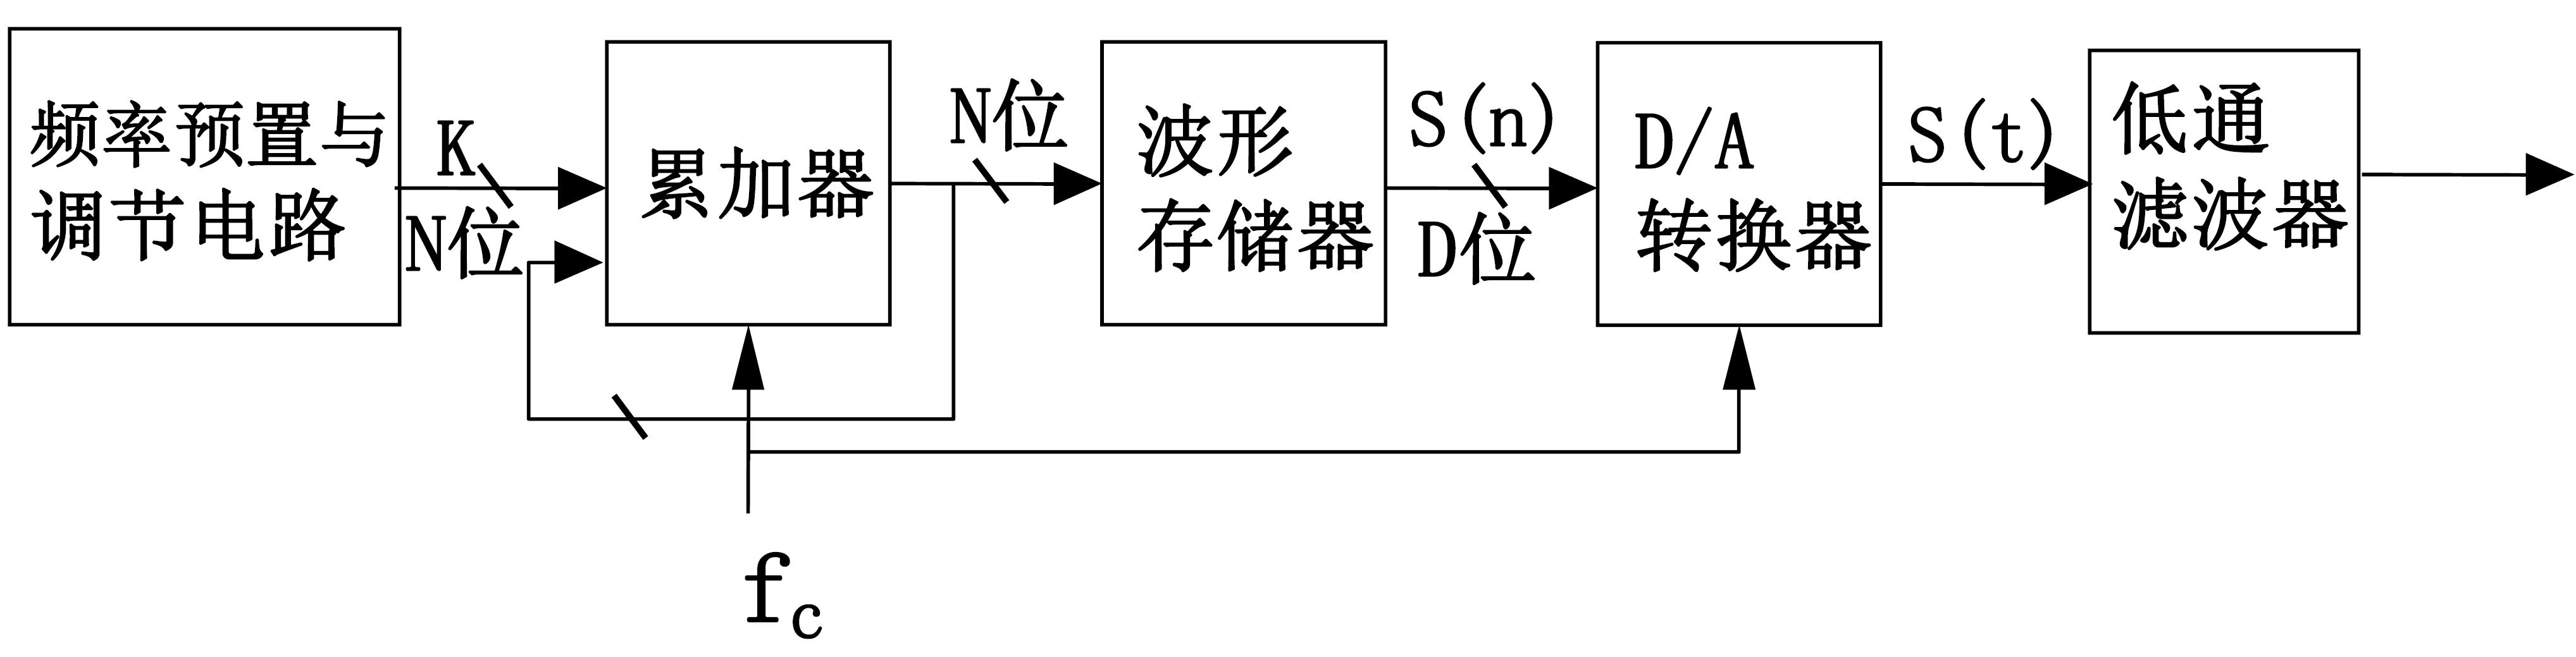
\includegraphics[width=\textwidth]{picture/yuanli.png}  %插入的图,包括JPG,PNG,PDF,EPS等,放在源文件目录下
	\caption{}  %图片的名称
	\label{fig:yuanli}   %标签,用作引用
\end{figure}
\subsection{频率预置与调节电路}
DDFS的输出频率为$$f_0=\frac{f_c K}{2^N}$$ \par
$f_0$为输出频率,$f_c$为时钟频率。当$K=1$时,DDFS输出最低频率(也即频率分辨率)为$\frac{f_c}{2^N}$ ;由Nyquist采样定理,DDFS的最大输出频率为$\frac{f_c}{2}$,也就是说K的最大值为$2^{N-1}$。\par因此,只要N足够大,DDFS可以得到很细的频率间隔。要改变DDFS的输出频率,只要改变频率控制字K即可。
\subsection{累加器}
\begin{figure}[htbp]
	\centering  
	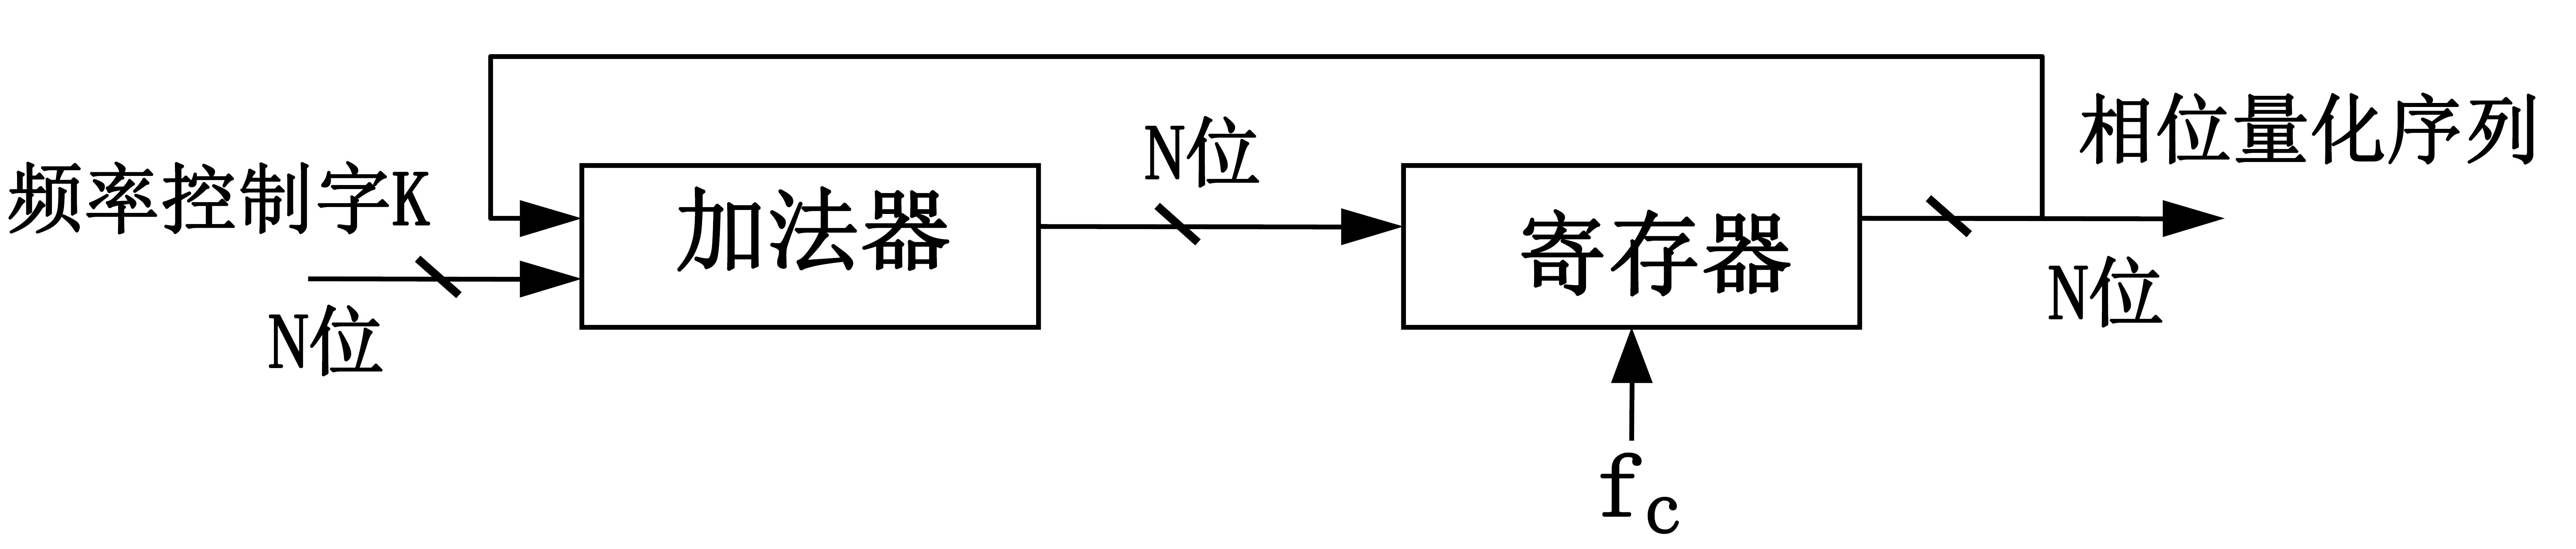
\includegraphics[width=\textwidth]{picture/yuanli2.png}  
	\caption{}  
	\label{fig:yuanli2}   
\end{figure}
如图\ref{fig:yuanli2},
累加器由N位加法器与N位寄存器级联构成。每收到一个时钟脉冲$f_C$,加法器便将频率控制字K与寄存器输出的累加相位数据相加,再把相加后的结果送至寄存器的数据输入端。寄存器将加法器在上一个时钟作用后所产生的相位数据反馈到加法器的输入端;使加法器在下一个时钟作用下继续与频率控制字进行相加。这样,相位累加器在时钟的作用下,进行相位累加。\par当相位累加器累加满量时就会产生一次溢出,完成一个周期性的动作,这个周期应为$$T_o=\frac{2^N}{K} T_c$$
\subsection{波形存储器}
\begin{figure}[htbp]
	\centering  
	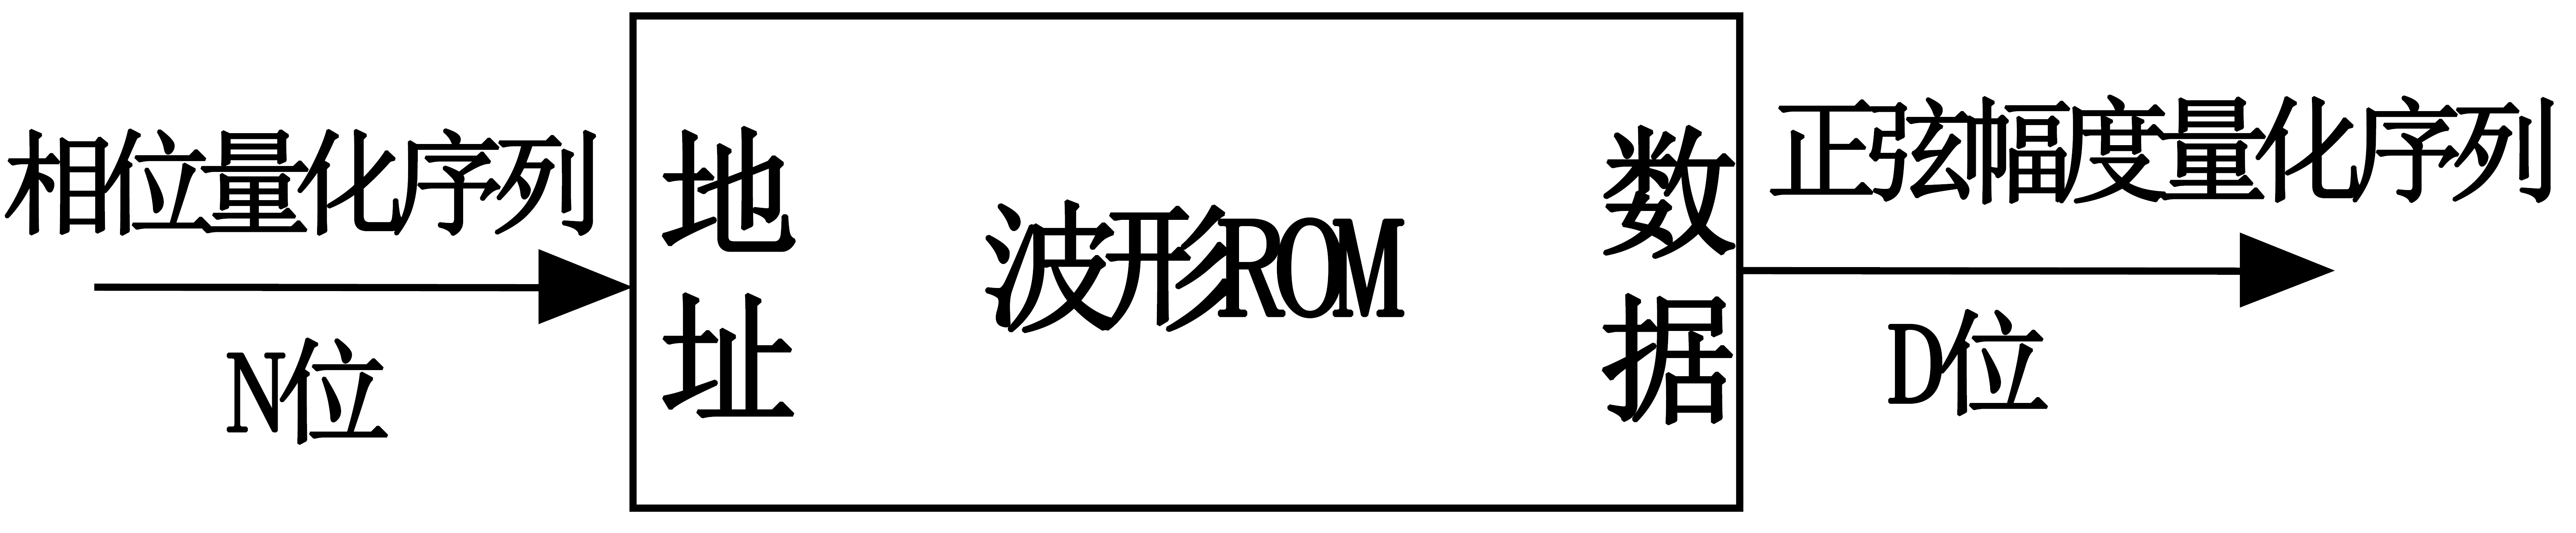
\includegraphics[width=0.8\textwidth]{picture/yuanli3.png}  
	\caption{}  
	\label{fig:yuanli3}   
\end{figure}
如图\ref{fig:yuanli3},
将累加器输出的数据作为波形存储器的地址,进行波形的相位-幅值转换,可在给定的时间上确定输出波形的幅值。\par N位的寻址ROM相当于把周期的波形信号离散成具有$2^N$个样值的序列,若波形ROM有D位数据位,则$2^N$个样值的幅值以D位二进制数值存在ROM中,按照地址的不同可以输出相应相位的波形信号的幅值。
\subsection{D/A转换器}
\begin{figure}[htbp]
	\centering  
	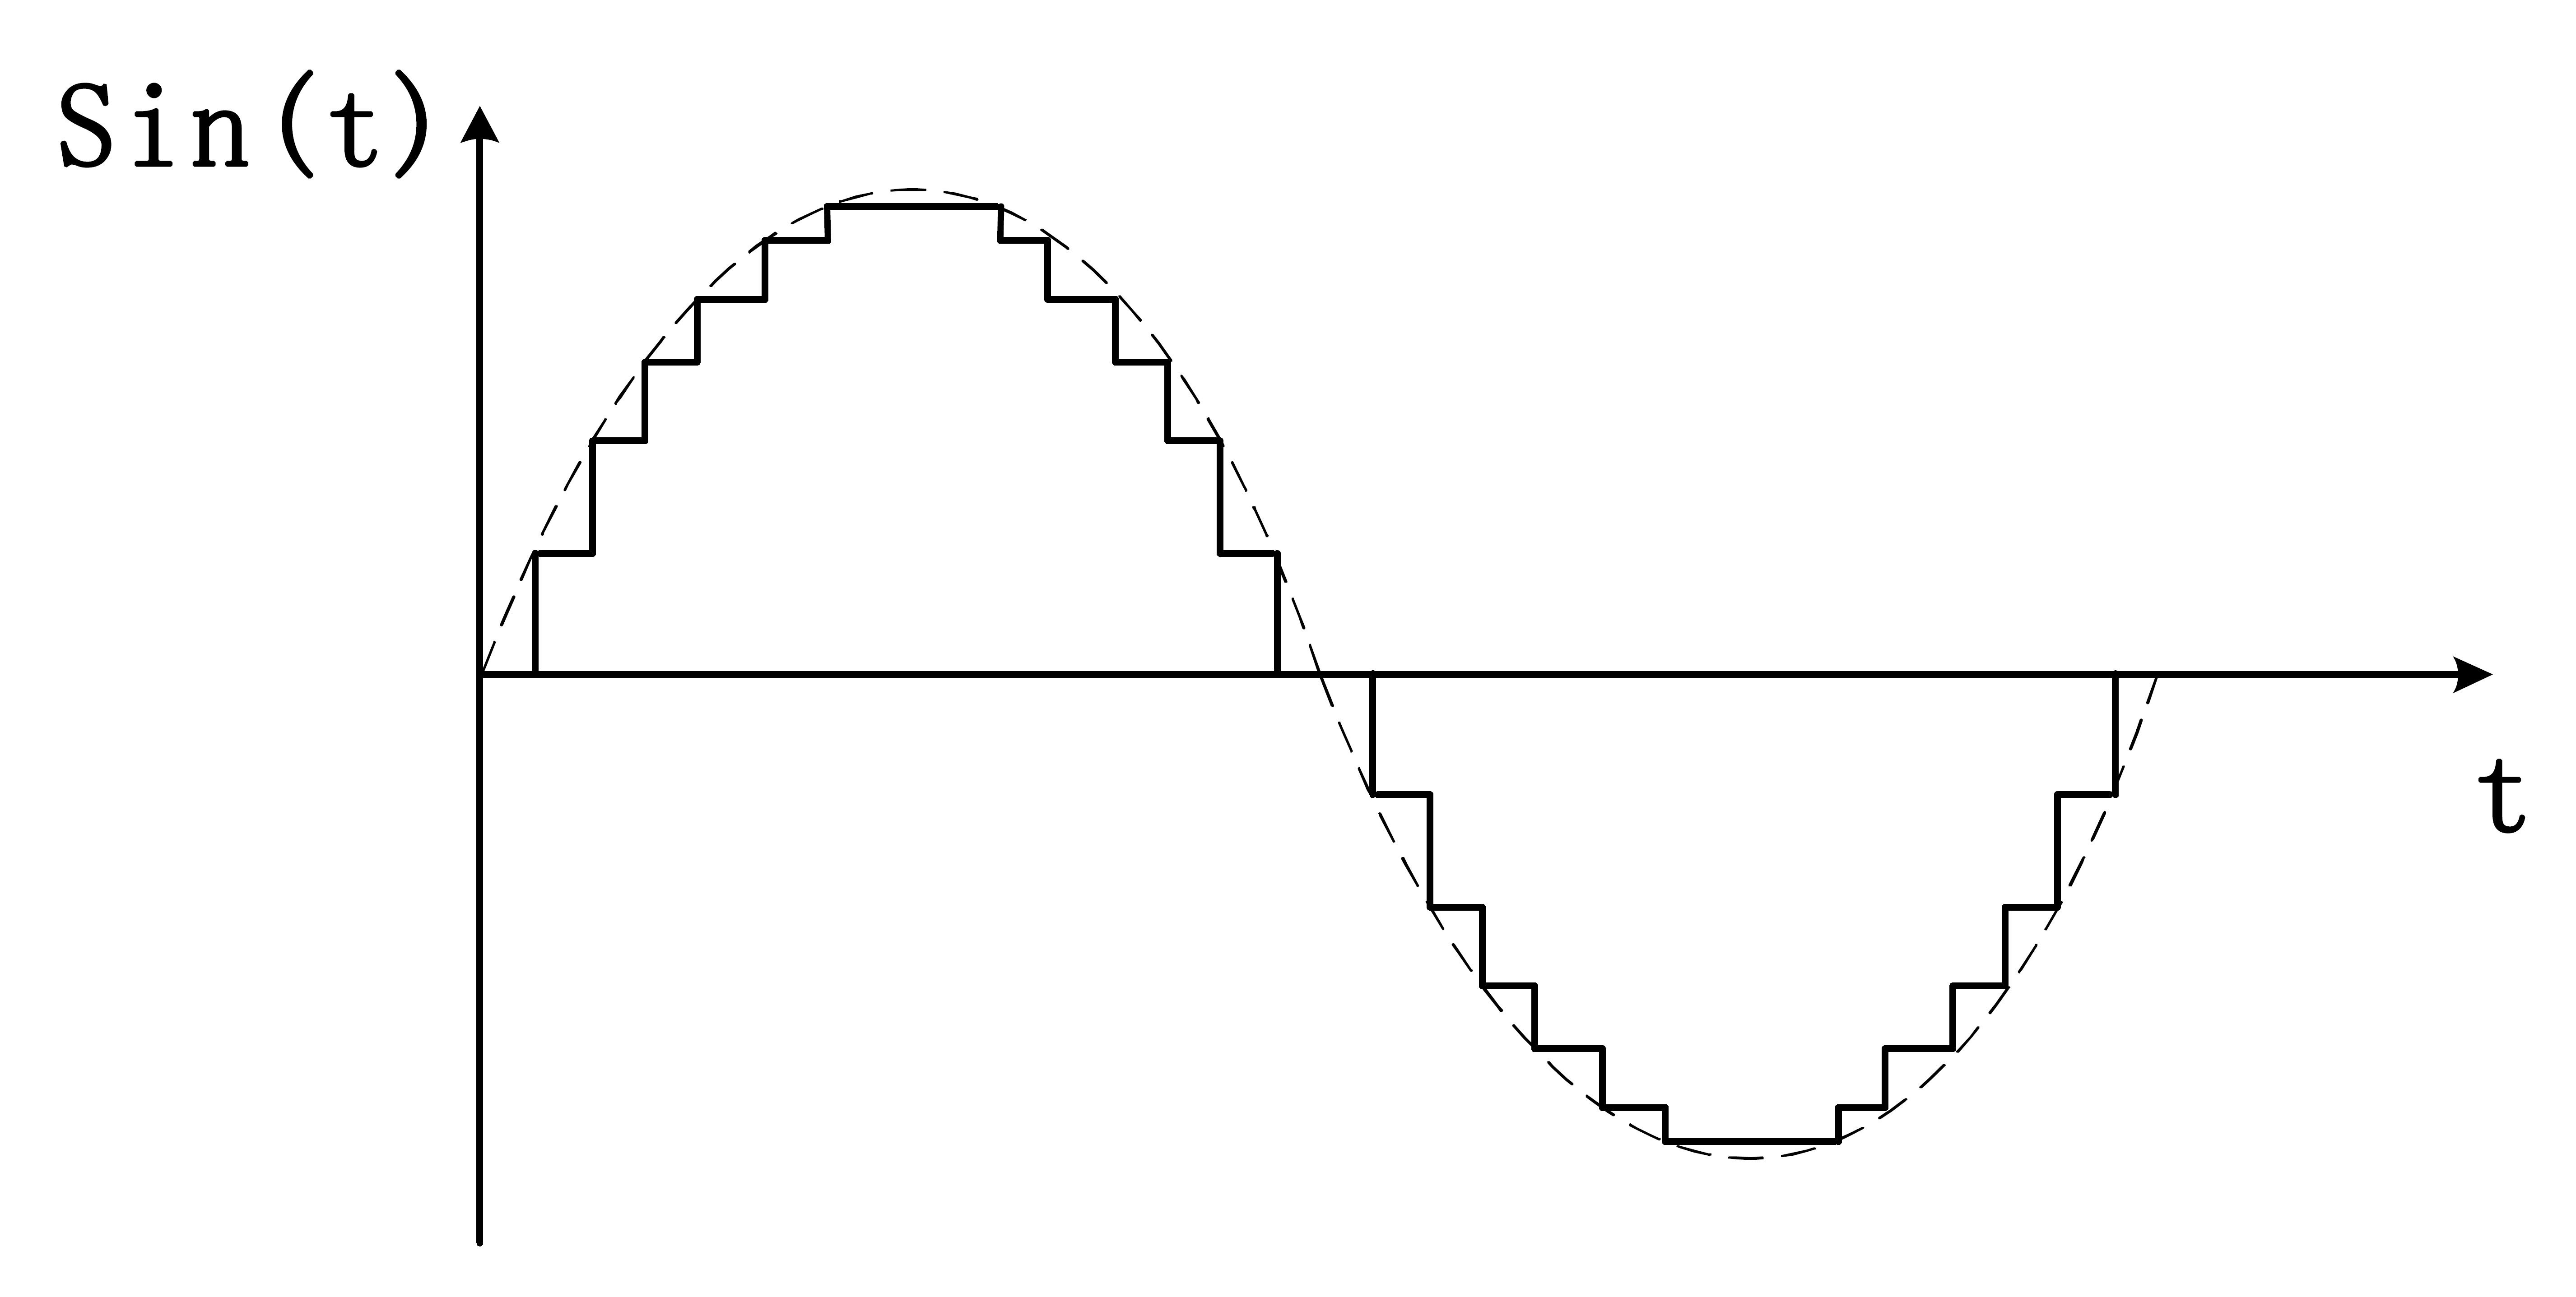
\includegraphics[width=0.7\textwidth]{picture/yuanli5.png}  
	\caption{}  
	\label{fig:yuanli5}   
\end{figure}
如图\ref{fig:yuanli5},
D/A转换器的作用是把已经合成的周期波的数字量转换成模拟量。波形幅度量化序列S(n)经D/A转换后变成了包络为周期波的阶梯波S(t), S(t)的周期为$$T=\frac{2^N}{K} T_C$$
\subsection{低通滤波器}
\begin{figure}[htbp]
	\centering  
	\includegraphics[width=\textwidth]{picture/yuanli6.png}  
	\caption{}  
	\label{fig:yuanli6}   
\end{figure}
如图\ref{fig:yuanli6},低通滤波器的作用是
滤除生成的阶梯形正弦波中的高频成分,将其变
成光滑的正弦波。
\section{各子模块设计原理}

\subsection{脉冲发生电路}
通过分频,将实验箱提供的48MHz的高频信号通过分频器变成所需的1Hz、0.5Hz和1KHz的信号,0.5Hz用于测频电路,1Hz用于计数,2Hz用于消颤,1KHz用于译码显示电路。
\subsubsection{VHDL分频原理}
对时钟信号进行上升沿检测,并记录检测的数(从 0 开始计数)。如果是 N 分频,每当计数到$\frac{N}{2}-1$时将信号翻转一次,将信号输出。
\subsubsection{分频模块}
相应的VHDL代码如下,由于要将48MHz分频出1Hz需要的截止时间过长,而分频原理其实是一致的,因此只要1MHz的分频结果正确,就可以认为分频无误,其仿真波形见图\ref{fig:fangzhenfenpin},封装图见图\ref{fig:fengzhuangfenpin}。
\begin{lstlisting}[language=VHDL]
LIBRARY IEEE;
USE IEEE.STD_LOGIC_1164.ALL;
ENTITY fenpin2 IS
PORT(clk:IN STD_LOGIC;
mhz:buffer STD_LOGIC;
hz1:buffer STD_LOGIC;
hz0_5:buffer STD_LOGIC;
hz2:buffer STD_LOGIC;
khz:buffer STD_LOGIC);
END fenpin2;
ARCHITECTURE beh OF fenpin2 IS
SIGNAL count:integer range 0 to 24;
SIGNAL count1:integer range 0 to 24000000;
SIGNAL count2:integer range 0 to 48000000;
SIGNAL count3:integer range 0 to 12000000;
SIGNAL count4:integer range 0 to 24000;
BEGIN
PROCESS(clk)
BEGIN
IF(clk='1')THEN
count<=count+1;
count1<=count1+1;
IF(count=23)THEN
count<=0;
mhz<=NOT mhz;
END IF;
IF(count1=23999999)THEN
count1<=0;
hz1<=NOT hz1;
END IF;
IF(count2=47999999)THEN
count2<=0;
hz0_5<=NOT hz0_5;
END IF;
IF(count3=11999999)THEN
count3<=0;
hz2<=NOT hz2;
END IF;
IF(count3=11999)THEN
count4<=0;
khz<=NOT khz;
END IF;
END IF;
END PROCESS;
END beh;

\end{lstlisting}

\begin{figure}[hp]
	\centering  
	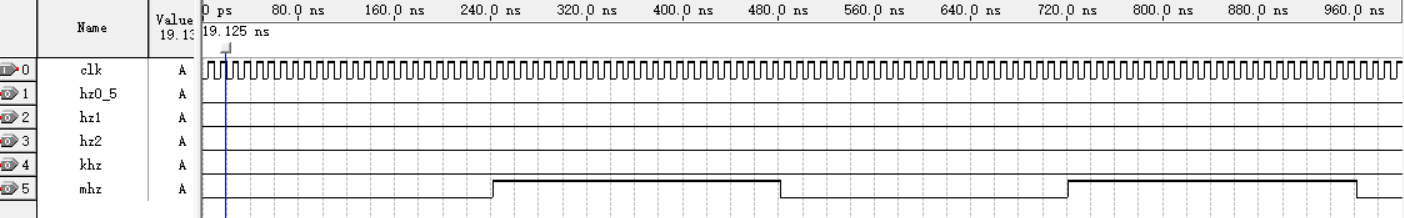
\includegraphics[width=\textwidth]{picture/fenpinfangz.png} 
	\caption{}
	\label{fig:fangzhenfenpin}   
\end{figure}
\begin{figure}[hp]
	\centering  
	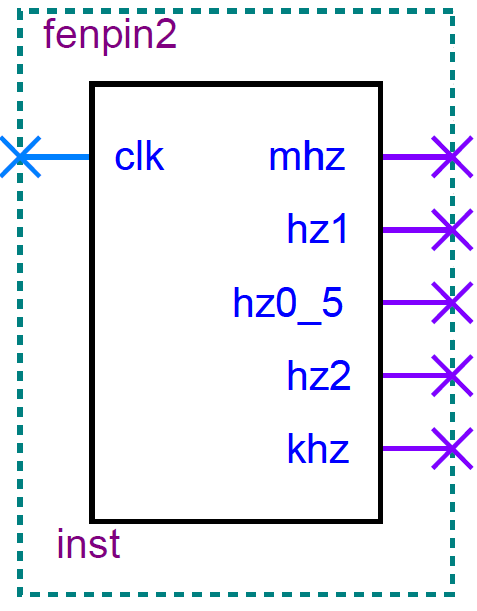
\includegraphics[width=0.3\textwidth]{picture/TIM20181212143832.png} 
	\caption{}
	\label{fig:fengzhuangfenpin}   
\end{figure}
\subsection{频率字、相位字产生电路}
\subsubsection{电路原理}
频率预置与调节电路的主要作用是实现频率控制量的输入,不变量K被称为相位增量,也叫频率控制字。DDFS的输出频率表达式为$$f_{out}=K\frac{f_c}{2^N}$$当K=1 时,输出最低频率为$\frac{f_c}{2^N}$,而DDFS的最高输出频率由Nyquist采样定理决定,即$f_out=\frac{f_c}{2}$。由于后续还需要测频并用4位显示,而4位可显示的最大频率对应的K值为40,于是我设计频率控制字K为一个模40的计数器。\par相位控制字和频率控制字在原理上没有区别,因此用同一个模块。
\subsubsection{模40模块}
相应的VHDL代码如下,其仿真波形见图\ref{fig:fangzhenmo40},封装图见图\ref{fig:fengzhuangmo40}。
\begin{lstlisting}[language=VHDL]
library ieee;
use ieee.std_logic_1164.all;
use ieee.std_logic_unsigned.all;
ENTITY mmo40 IS 
 PORT
    ( en   :IN  std_logic;
      clear:IN  std_logic;
      clk  :IN  std_logic;
      cout :out  std_logic;
      qh   :buffer std_logic_vector(3 downto 0);
      ql   :buffer std_logic_vector(3 downto 0)
    );
END mmo40;
ARCHITECTURE behave OF mmo40 IS
BEGIN
cout<='1'when(qh="0011"and ql="1001"and en='0')else'0'; 

   PROCESS(clk,clear)
     BEGIN
       IF(clear='1')THEN
                qh<="0000";
                ql<="0000";
              ELSIF(clk'EVENT AND clk='1')THEN
                 if(en='0')then
                          if((ql=9 and qh=3) or ql=9) then
                                ql<="0000";
                               if(qh=3)then
                                  qh<="0000";
                                   else
                                  qh<=qh+1;
                                end if;
                               else
                               ql<=ql+1;
                              end if;
                             end if;
                     END IF;
             END PROCESS;
           END behave;

\end{lstlisting}
\begin{figure}[hp]
	\centering  
	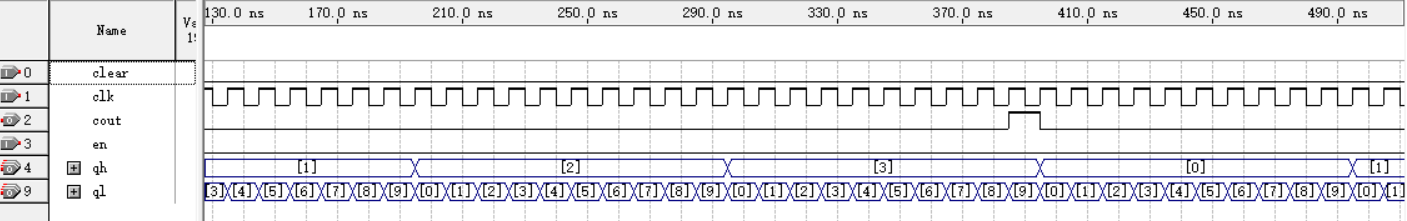
\includegraphics[width=\textwidth]{picture/mo40box.png} 
	\caption{}
	\label{fig:fangzhenmo40}   
\end{figure}
\begin{figure}[hp]
	\centering  
	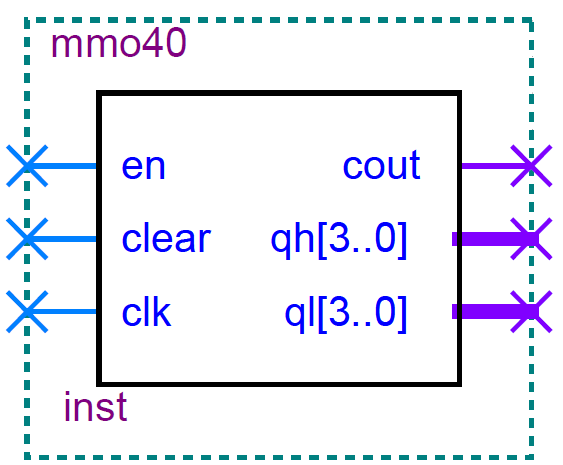
\includegraphics[width=0.3\textwidth]{picture/mo40fz.png} 
	\caption{}
	\label{fig:fengzhuangmo40}   
\end{figure}
\subsection{BCD码转二进制电路}
\subsubsection{电路作用}
由于BCD码无法直接用乘法器或加法器进行运算,因此需将BCD转二进制,使频率字、相位字得出的BCD码转换为二进制。
\subsubsection{BCD码转二进制模块}
相应的VHDL代码如下,封装图见图\ref{fig:fengzhuangBCD}。
\begin{lstlisting}[language=VHDL]
entity BCD is
port(d0,d1:in integer range 0 to 9;
binary:out integer range 0 to 63);
end BCD;
architecture one of BCD is
begin
binary<=d0+10*d1;
end one;
\end{lstlisting}
\begin{figure}[hp]
	\centering  
	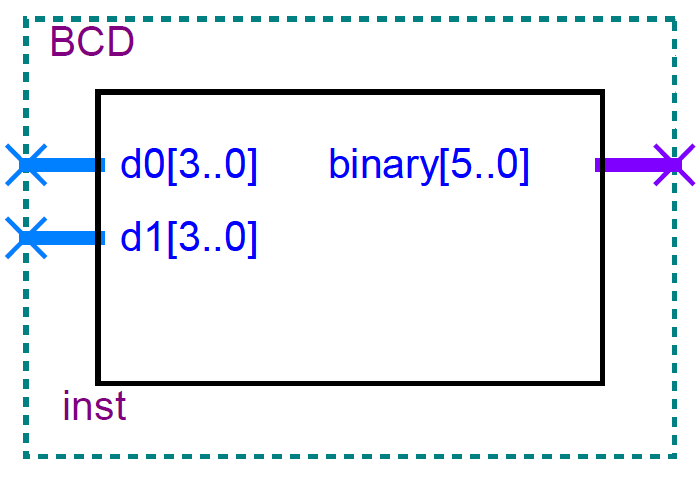
\includegraphics[width=0.3\textwidth]{picture/bcd.png} 
	\caption{}
	\label{fig:fengzhuangBCD}   
\end{figure}
\subsection{累加器}
累加器由N位加法器N位寄存器构成。\par如图\ref{fig:yuanli2},
其作用是,每接收一个时钟clk,加法器就将频率控制字 与累加寄存器输出的累加相位数据相加,相加的结果又反馈送至累加寄存器的数据输入端,以使加法器在下一个时钟脉冲的作用下继续与频率控制字相加。这样,相位累加器在时钟作用下,不断对频率控制字进行线性相位累加。
\subsubsection{加法器模块}
相应的VHDL代码如下,其仿真波形见图\ref{fig:fangzhenadd},封装图见图\ref{fig:fengzhuangadd}。
\begin{lstlisting}[language=VHDL]
LIBRARY ieee;
USE ieee.std_logic_1164.ALL;
USE ieee.std_logic_unsigned.ALL;

ENTITY adder12 IS 
PORT(A:IN std_logic_vector(11 DOWNTO 0);
     K:IN std_logic_vector(5 DOWNTO 0);
     S:OUT std_logic_vector(11 DOWNTO 0));

END adder12;
    
ARCHITECTURE done OF adder12 IS
 signal sum:std_logic_vector(11 downto 0);
BEGIN
  sum<=K+A;
  s<=sum;
END done;
\end{lstlisting}
\begin{figure}[hp]
	\centering  
	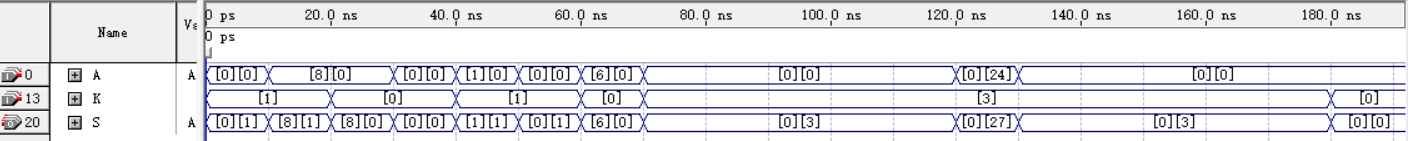
\includegraphics[width=\textwidth]{picture/TIM20181212152917.png} 
	\caption{}
	\label{fig:fangzhenadd}   
\end{figure}
\begin{figure}[hp]
	\centering  
	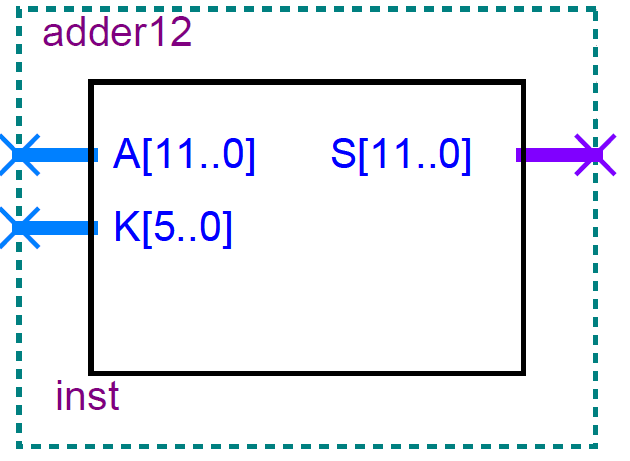
\includegraphics[width=0.3\textwidth]{picture/add.png} 
	\caption{}
	\label{fig:fengzhuangadd}   
\end{figure}
\subsubsection{寄存器模块}
相应的VHDL代码如下,其封装图见图\ref{fig:fengzhuangreg}。
\begin{lstlisting}[language=VHDL]
LIBRARY ieee;
USE ieee.std_logic_1164.ALL;
USE ieee.std_logic_unsigned.ALL;

ENTITY register_12 IS 
PORT(D:IN std_logic_vector(11 DOWNTO 0);
     CLK:IN std_logic;
     Q:OUT std_logic_vector(11 DOWNTO 0));

END register_12;

ARCHITECTURE register_12_arch OF register_12 IS
BEGIN
 PROCESS(CLK)
  BEGIN
    IF(CLK'EVENT AND CLK='1') THEN
        Q<=D;
    END IF;
  END PROCESS;
END register_12_arch;
\end{lstlisting}
\begin{figure}[hp]
	\centering  
	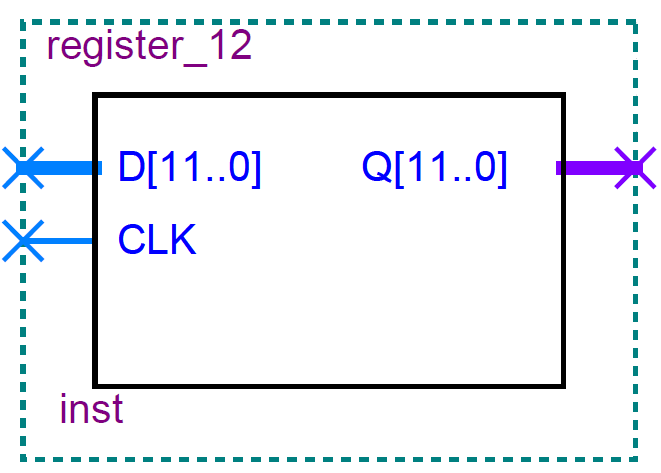
\includegraphics[width=0.3\textwidth]{picture/reg.png} 
	\caption{}
	\label{fig:fengzhuangreg}   
\end{figure}
\subsection{波形存储器与波形选择电路}
\subsubsection{波形文件的生成}
利用EXCEL的函数,可产生正弦函数值,计算要产生4096个数据所需要的角频率和幅值,再利用ROUND函数取整,代码为$$=ROUND((SIN(2*PI()/4096*(\$A1))+1)*511,0)$$,就可以产生离散的数据,部分数据见表\ref{tab:sin},将EXCEL的数据复制到txt文档,替换表格间空格,再更改文件名,可以得到mif文件。\par同理,可得到其他波形的mif文件。\par利用lpm\_rom进行波形封装,得到正余弦、方波、锯齿波、三角波的ROM封装文件,类似图\ref{fig:sin}。
\begin{table}[htbp]
\centering
\caption{}
\label{tab:sin}
\begin{tabular}{cccc}
\hline
0  & : & 511 & ; \\
1  & : & 512 & ; \\
2  & : & 513 & ; \\
3  & : & 513 & ; \\
4  & : & 514 & ; \\
5  & : & 515 & ; \\
6  & : & 516 & ; \\
7  & : & 516 & ; \\
8  & : & 517 & ; \\
9  & : & 518 & ; \\
10 & : & 519 & ; \\
11 & : & 520 & ; \\
12 & : & 520 & ; \\
13 & : & 521 & ; \\
14 & : & 522 & ; \\
15 & : & 523 & ; \\
16 & : & 524 & ; \\
17 & : & 524 & ; \\
18 & : & 525 & ; \\
19 & : & 526 & ; \\
20 & : & 527 & ; \\
21 & : & 527 & ; \\
22 & : & 528 & ; \\
23 & : & 529 & ; \\
24 & : & 530 & ;\\\hline
\end{tabular}
\end{table}
\begin{figure}[hp]
	\centering  
	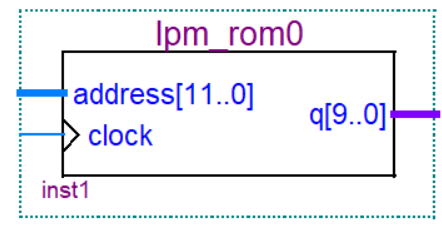
\includegraphics[width=0.3\textwidth]{picture/sin.png} 
	\caption{}
	\label{fig:sin}   
\end{figure}
\subsubsection{波形选择模块}
通过ipm\_mux元件构成波形选择电路,原理电路见图\ref{fig:xuanze},封装图见图\ref{fig:fengzhuangxuanze}。
\begin{figure}[hp]
	\centering  
	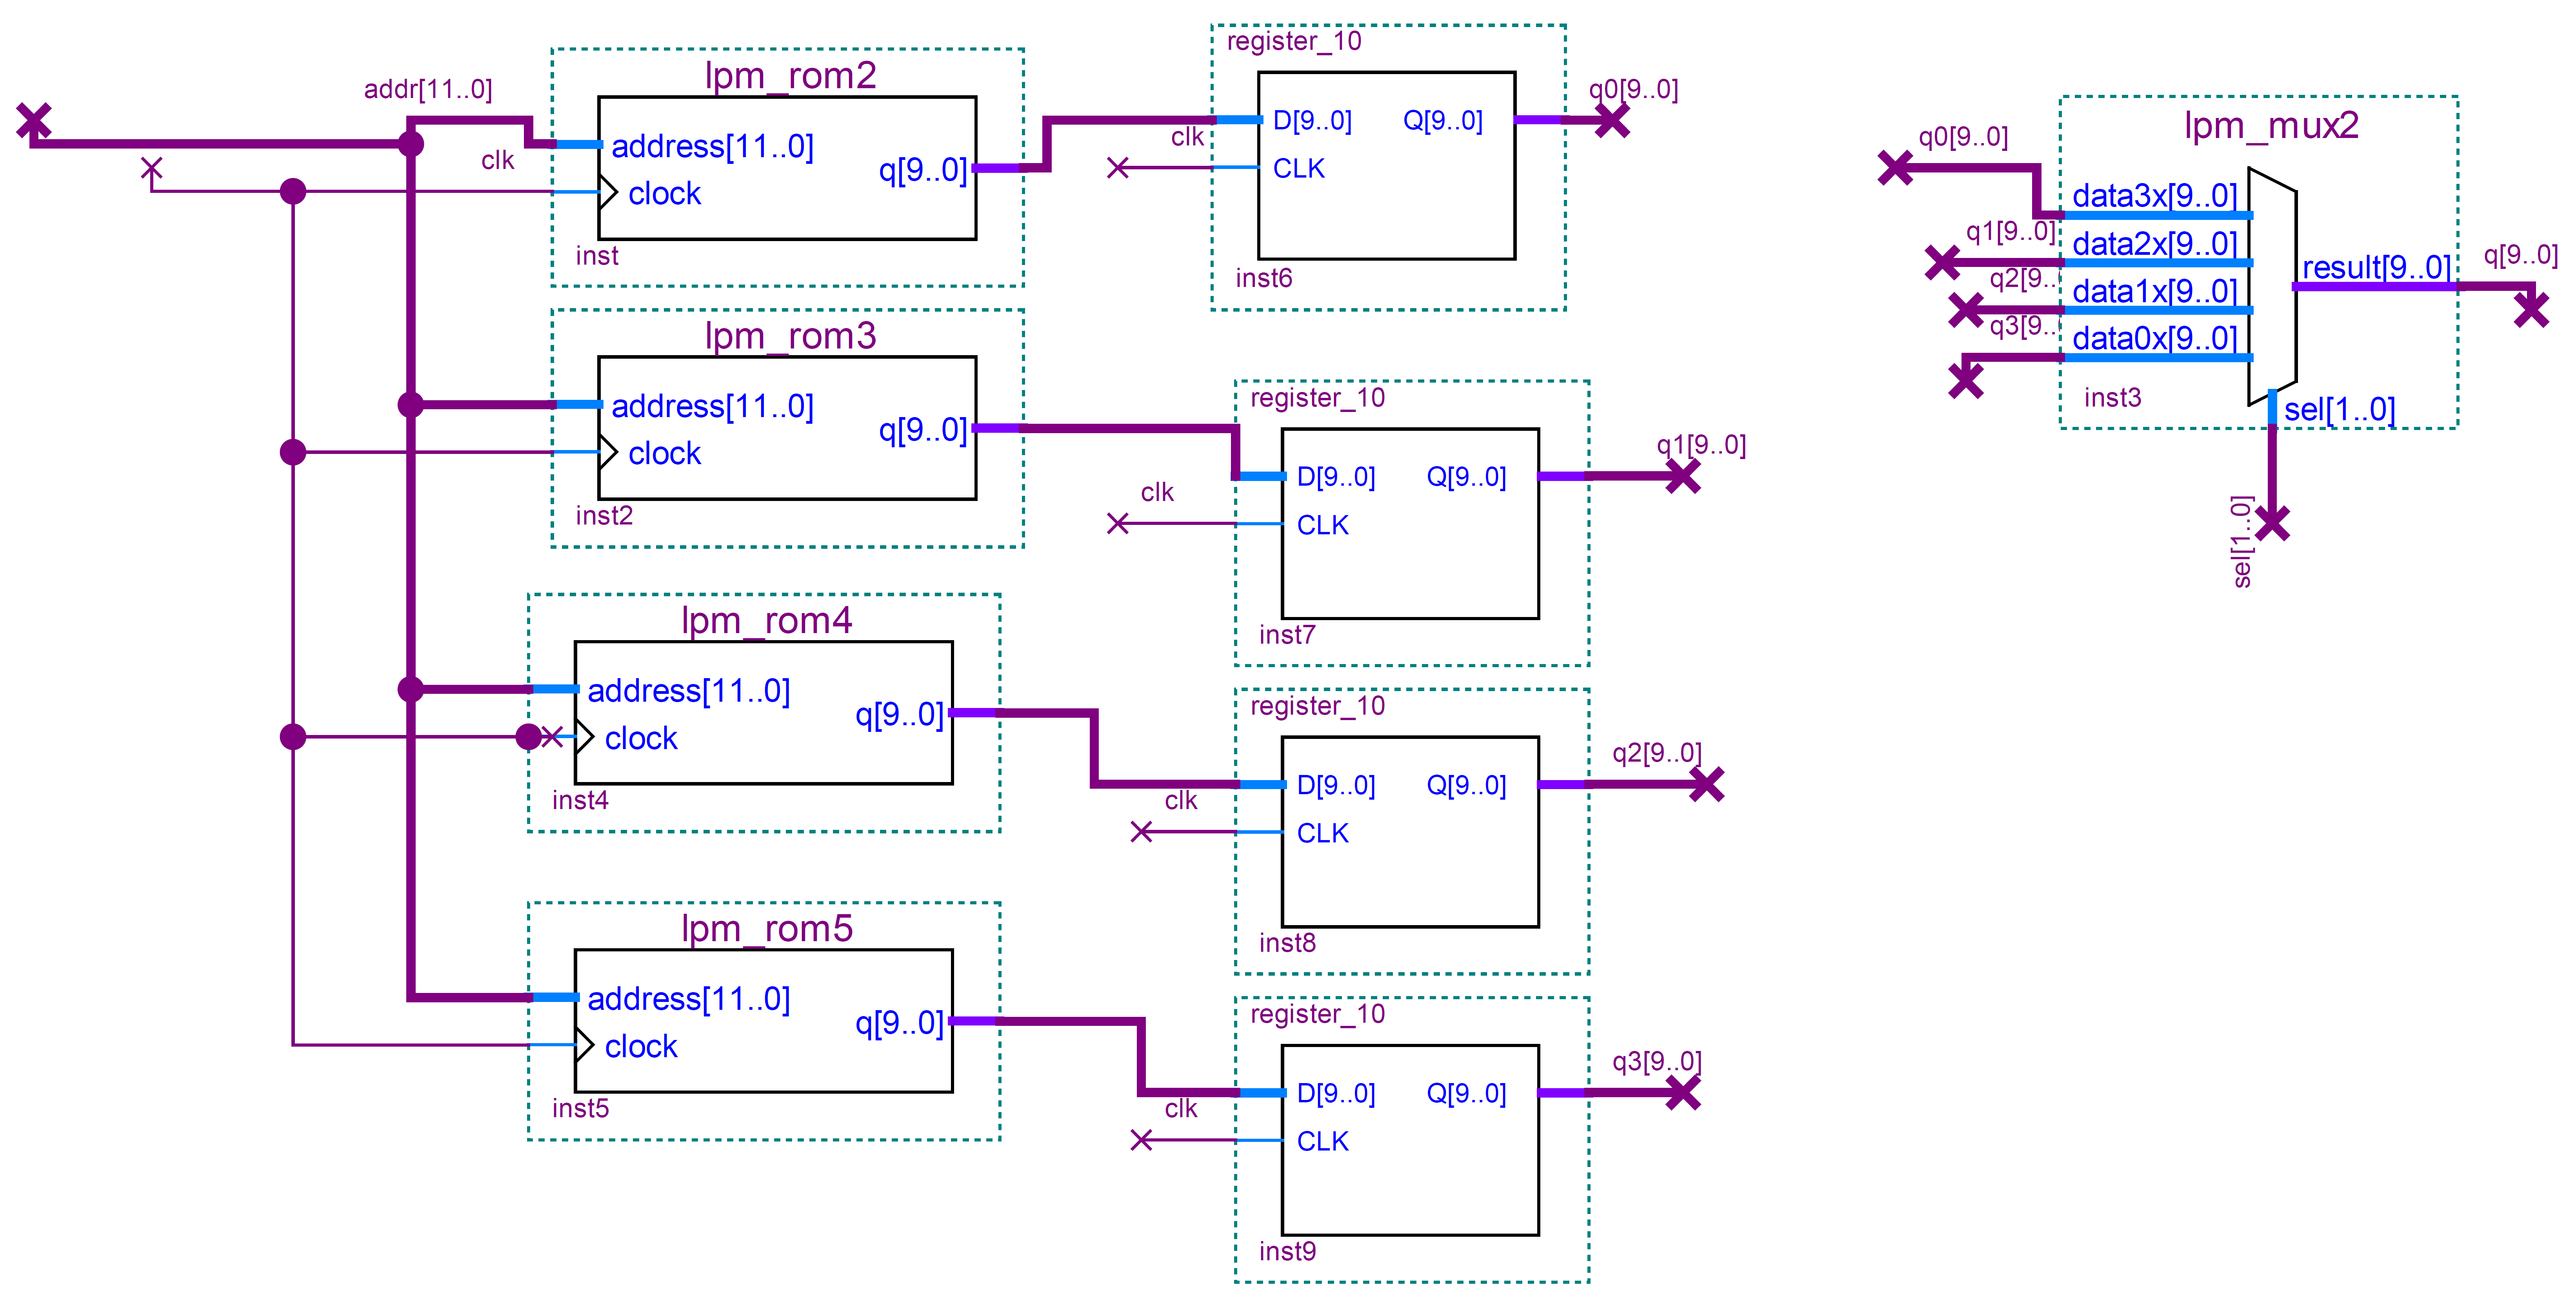
\includegraphics[width=\textwidth]{picture/xuanze.png} 
	\caption{}
	\label{fig:xuanze}   
\end{figure}
\begin{figure}[hp]
	\centering  
	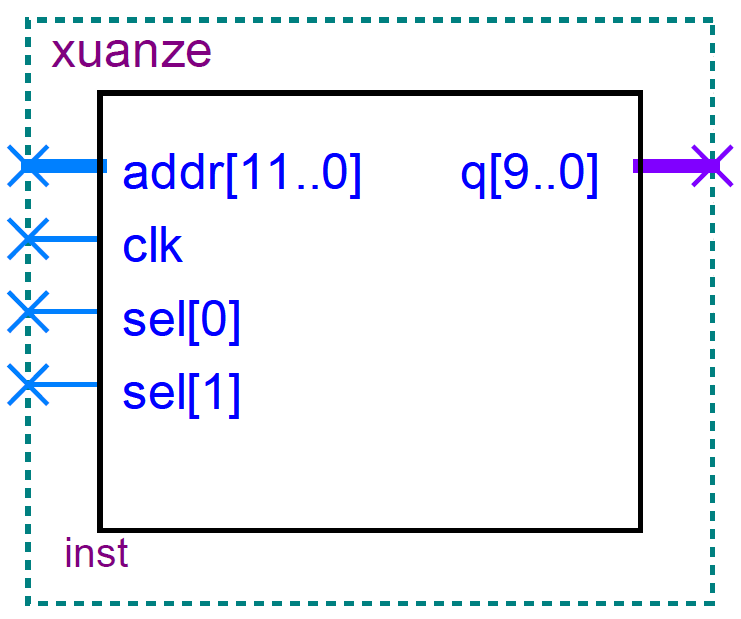
\includegraphics[width=0.3\textwidth]{picture/xuanzefz.png} 
	\caption{}
	\label{fig:fengzhuangxuanze}   
\end{figure}
\subsection{消颤电路}
由于开关的接通和关闭有可能产生毛刺,为了消除开关带来的竞争冒险,需要引入消颤模块。
\subsubsection{消颤电路原理}
通过一个D触发器对开关信号进行延时,从而得到稳定可靠的开关信号。
\subsubsection{消颤模块}
原理电路见图\ref{fig:xiaochan},封装图见图\ref{fig:fengzhuangxiaochanfz}。
\begin{figure}[hp]
	\centering  
	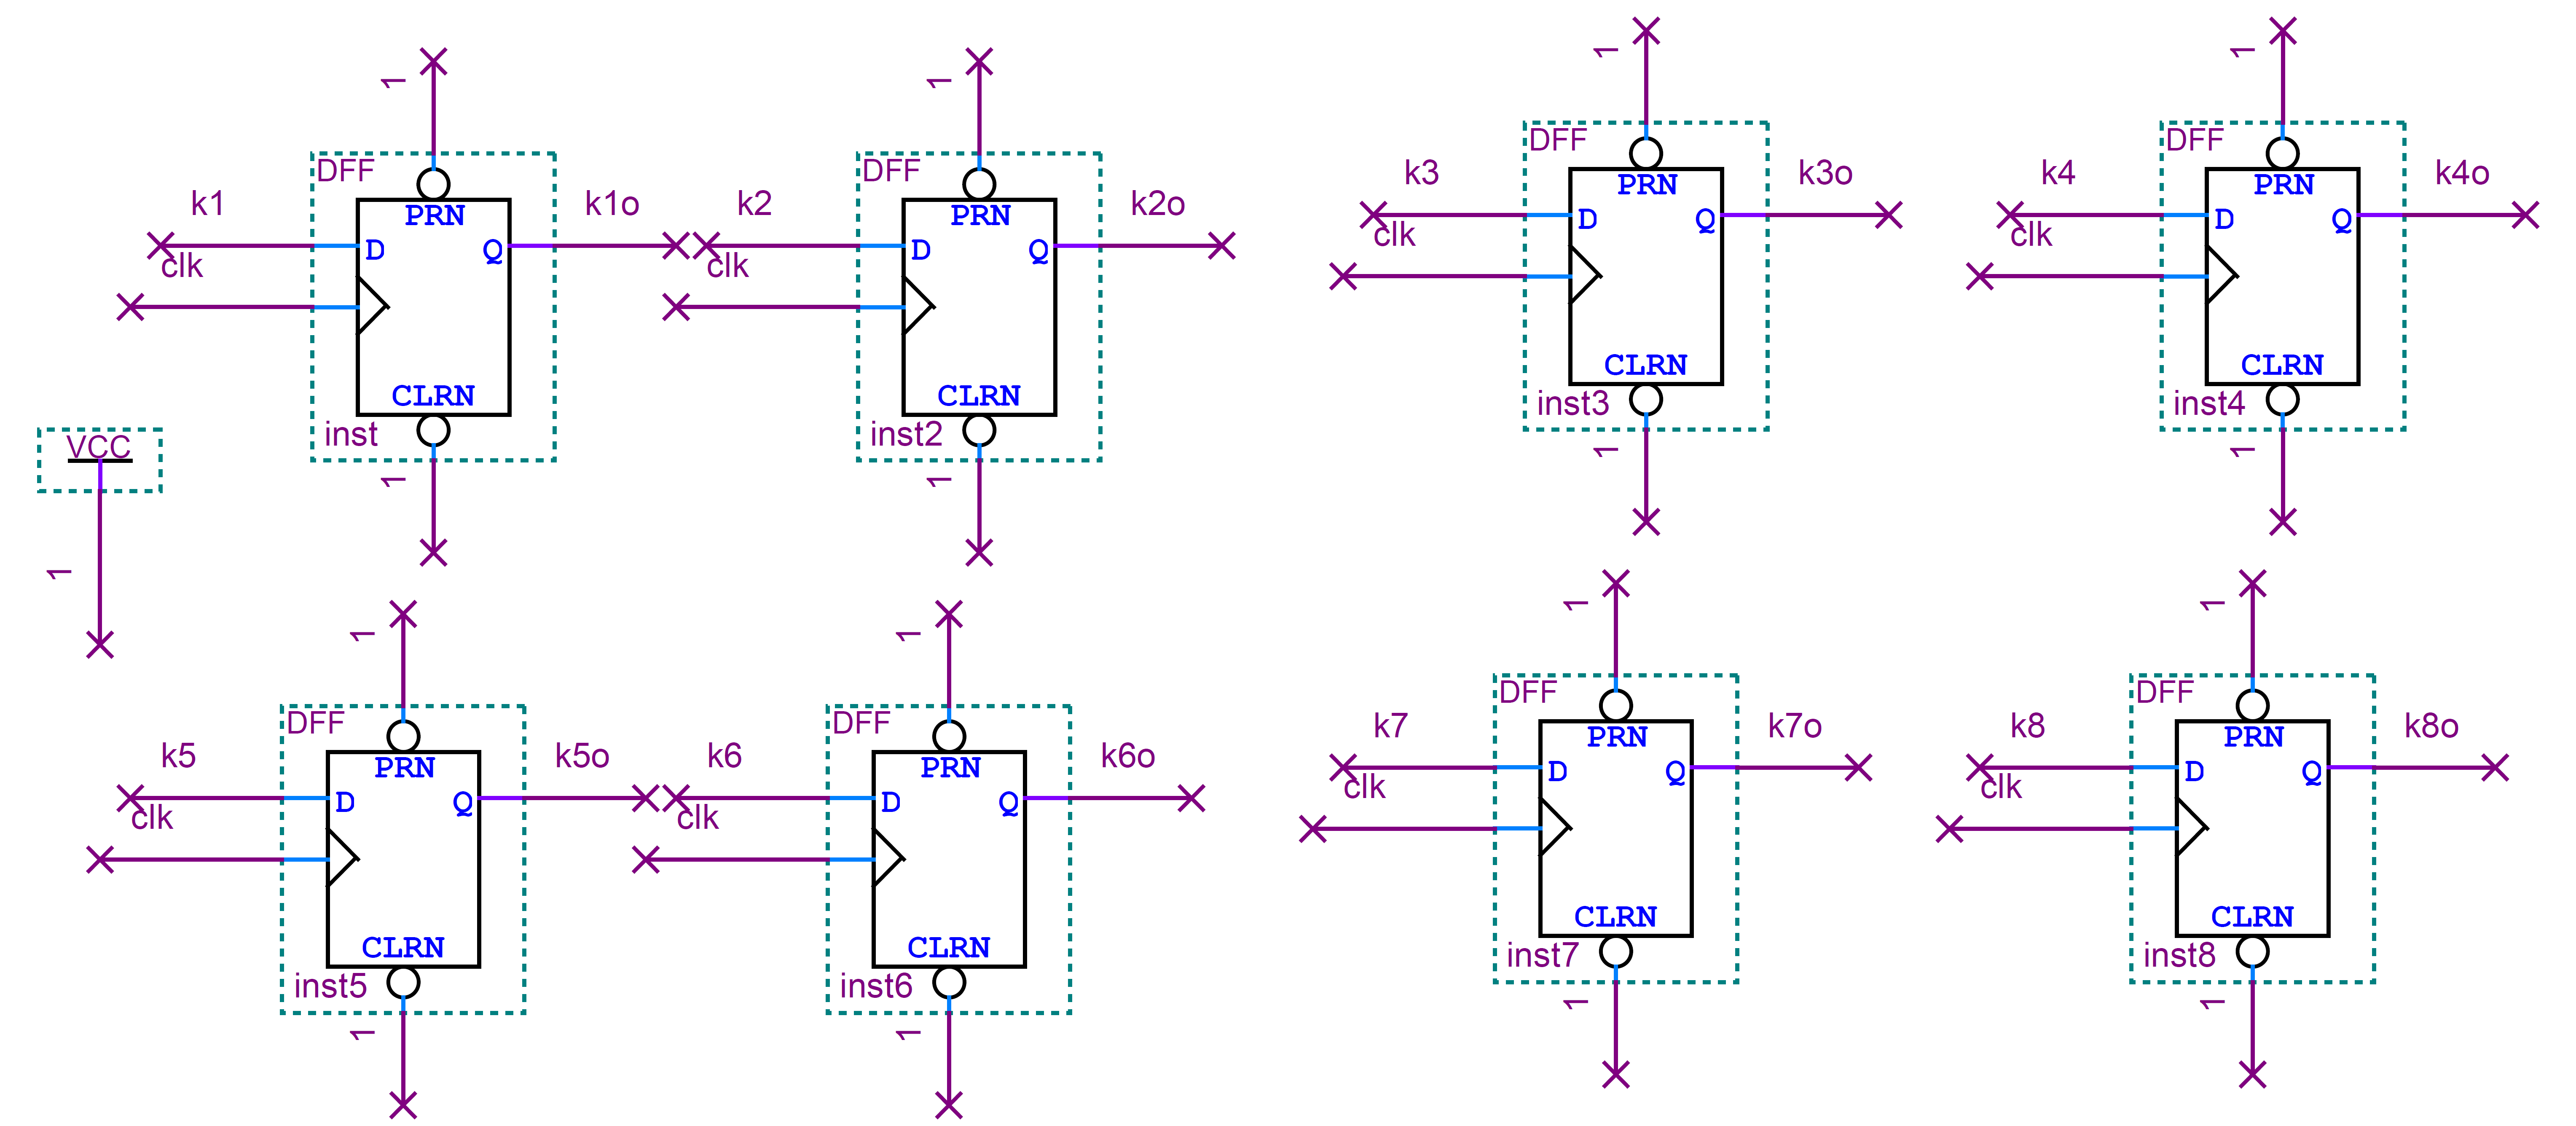
\includegraphics[width=\textwidth]{picture/xiaochan.png} 
	\caption{}
	\label{fig:xiaochan}   
\end{figure}
\begin{figure}[hp]
	\centering  
	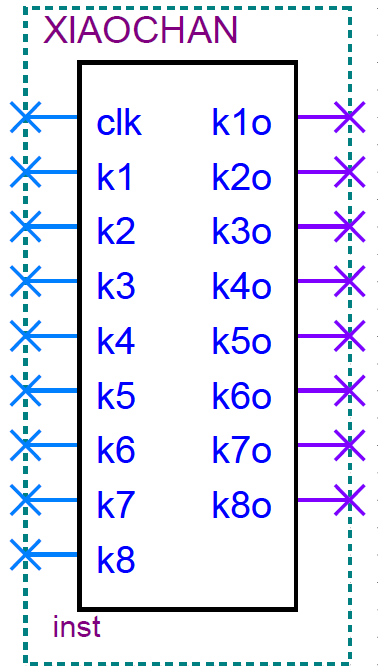
\includegraphics[width=0.3\textwidth]{picture/xiaochanfz.png} 
	\caption{}
	\label{fig:fengzhuangxiaochanfz}   
\end{figure}
\subsection{测频电路}
\subsubsection{测频原理}
测频就是计算1秒钟内脉冲的个数。我们利用计数器和锁存器实现这一功能。由于累加器以频率控制字K为间隔,从0-4095计数,当累加器满量时就会产生一次溢出,完成一次周期性的动作,这个周期也就是DDFS信号的一个频率周期,因此,将累加器的最高位作为测频电路技术器的脉冲。\par
如图\ref{fig:cepinyuanli},将0.5Hz脉冲送入锁存器的时钟端,0.5Hz反相延时后的脉冲送入计数器的清零端。这样就使计数器在2s的脉冲周期内,1s内清零,1s内计数。由于锁存器的脉冲和计数器的脉冲是反相的,且有一定的延时,所以当锁存器有效脉冲来到时,计数器是清零状态,锁存器就锁存前1s内计数器的计数信号。这样就完成了1s内的脉冲计数,再将锁存器的输出送入译码显示电路,就可以在数码管上显示波形频率了。
\begin{figure}[hp]
	\centering  
		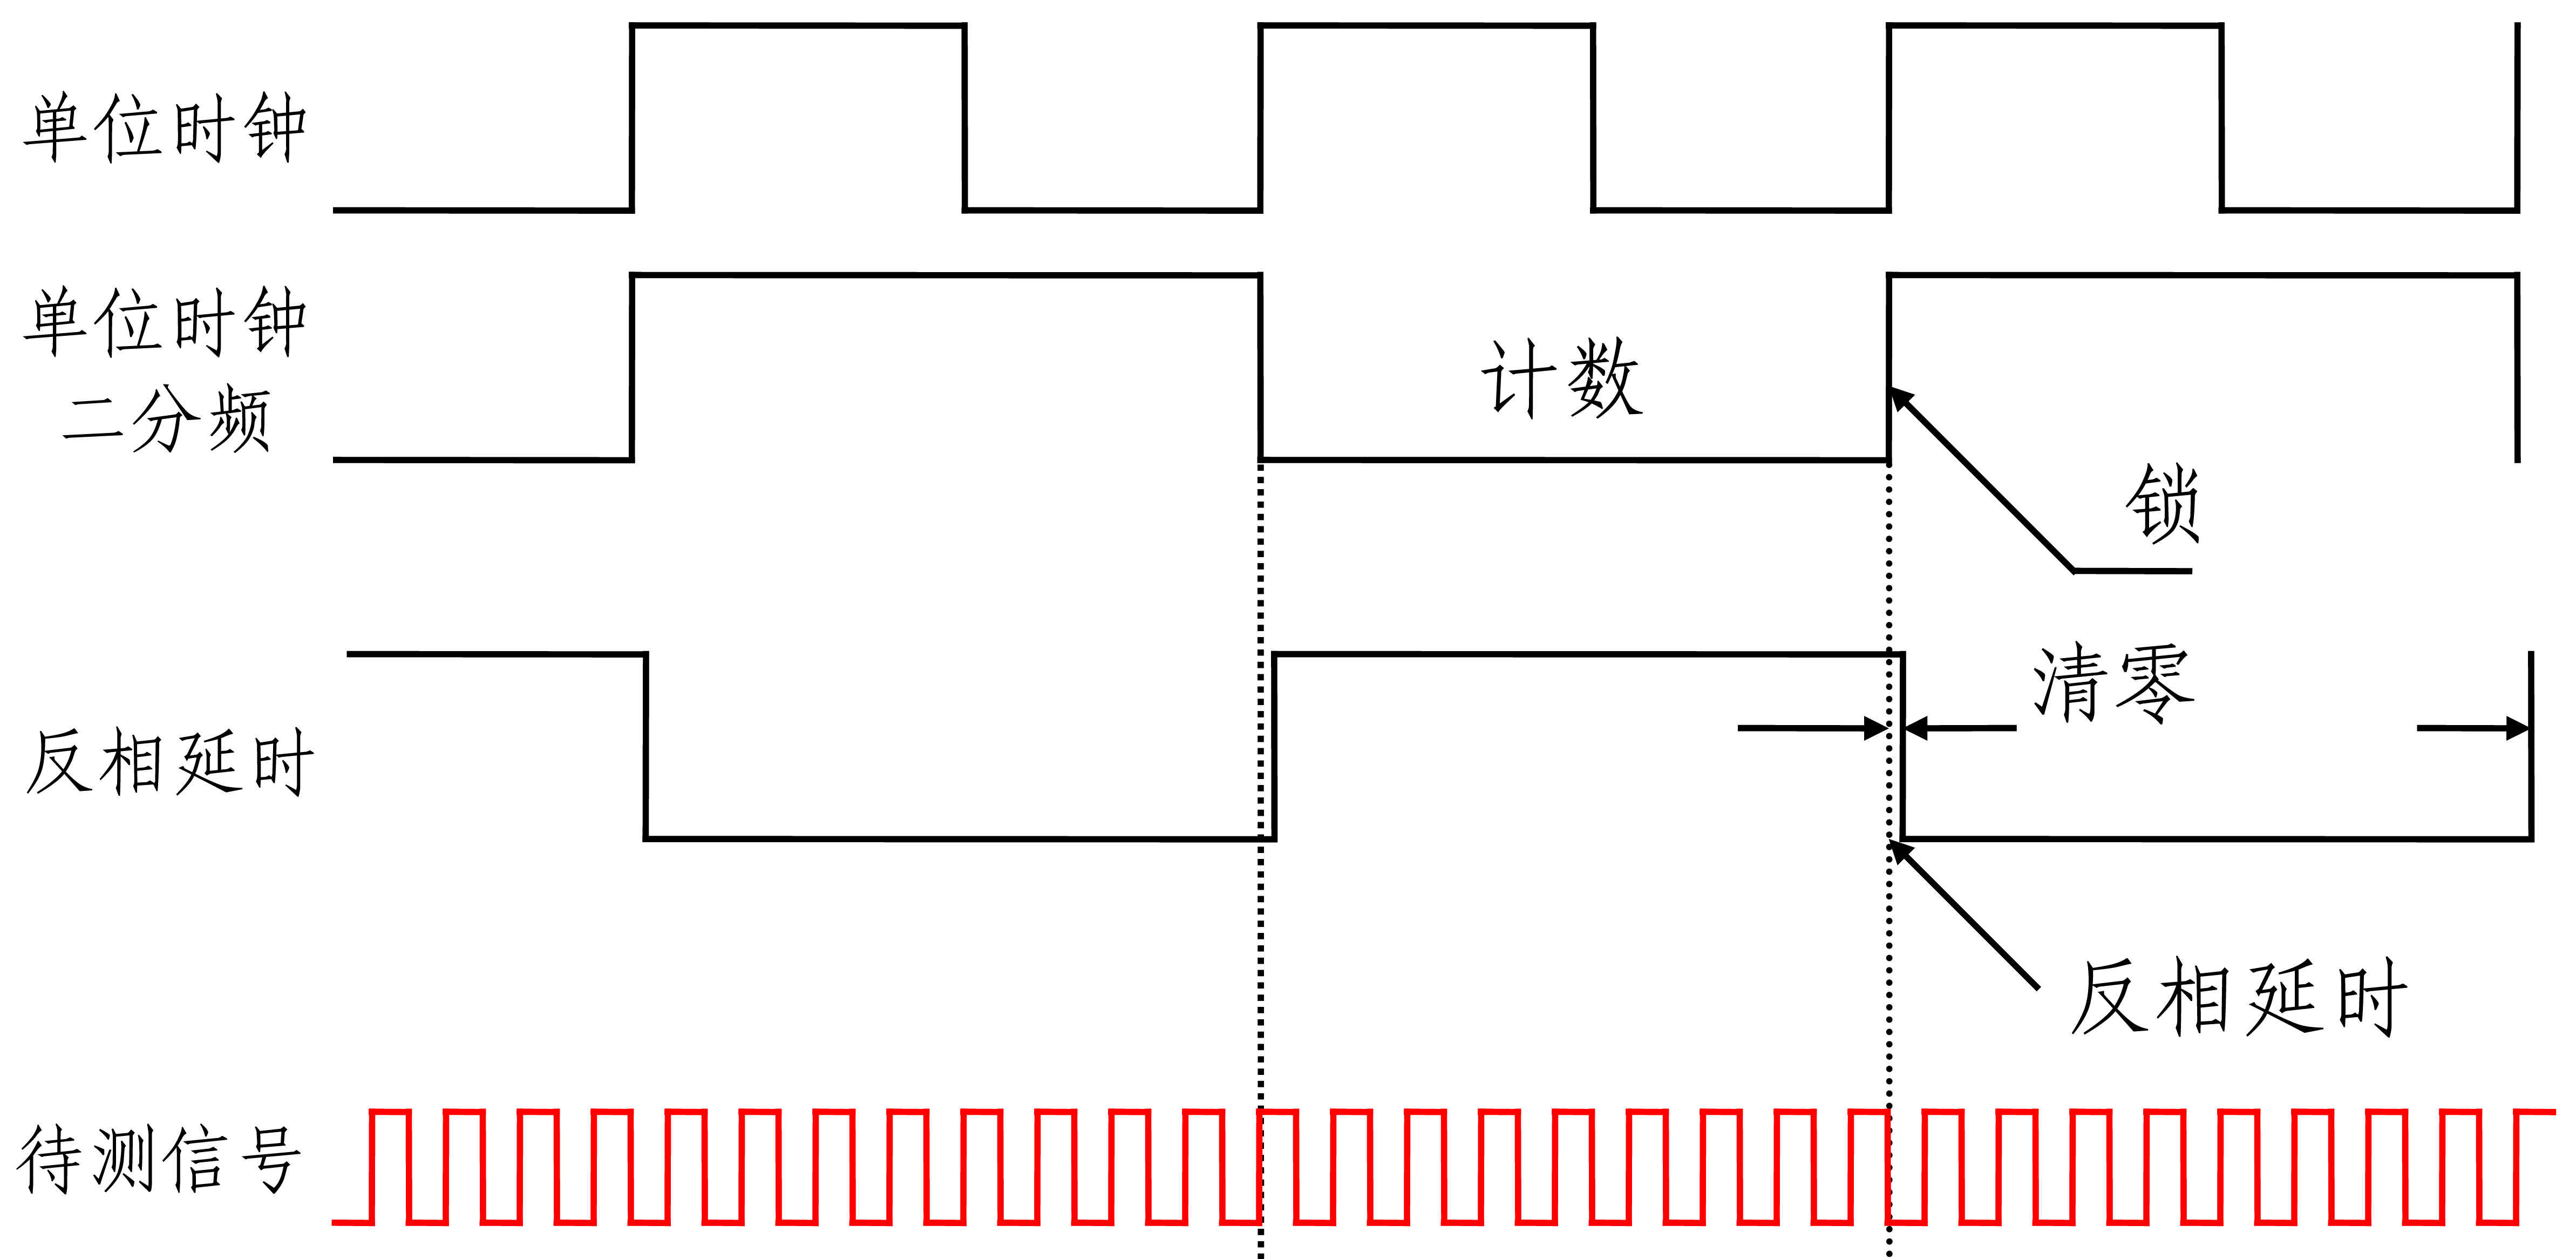
\includegraphics[width=\textwidth]{picture/image120.png} 
	\caption{}
	\label{fig:cepinyuanli}   
\end{figure}
\subsubsection{测频模块}
测频电路的原理电路见图\ref{fig:cepin},封装图见图\ref{fig:fengzhuangcepin}。
\begin{figure}[hp]
	\centering  
	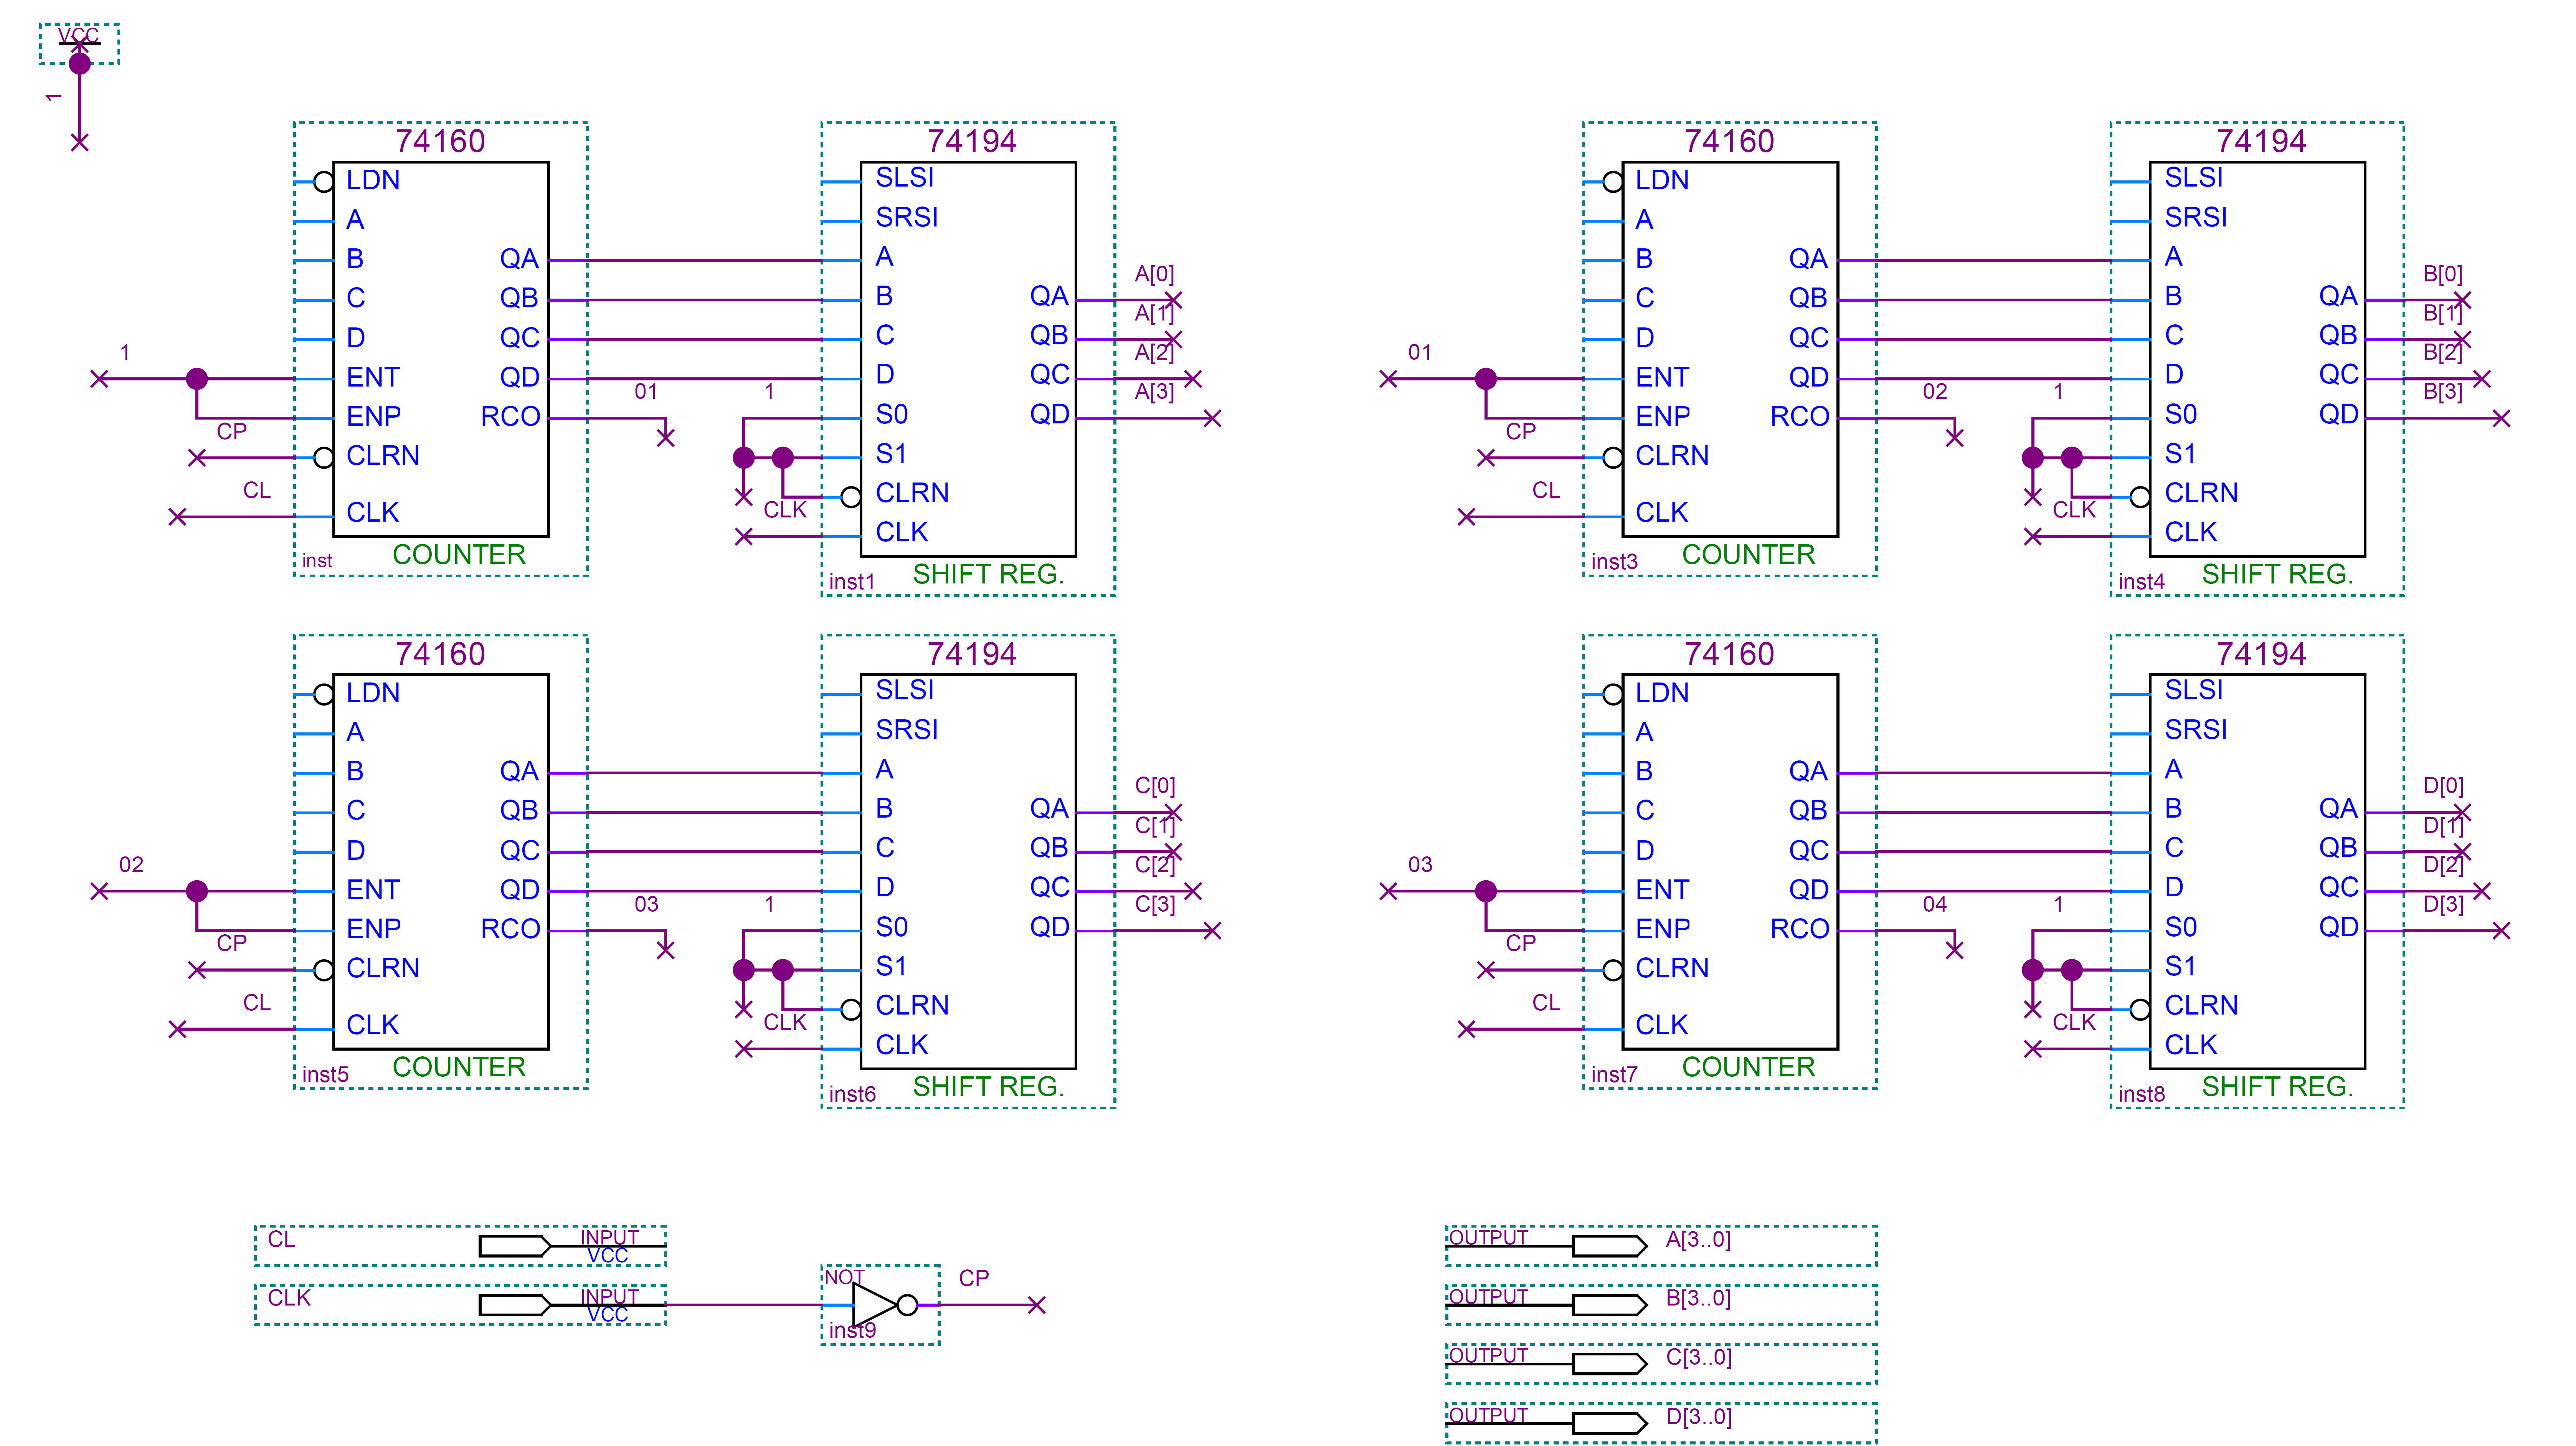
\includegraphics[width=\textwidth]{picture/cepin.png} 
	\caption{}
	\label{fig:cepin}   
\end{figure}
\begin{figure}[hp]
	\centering  
	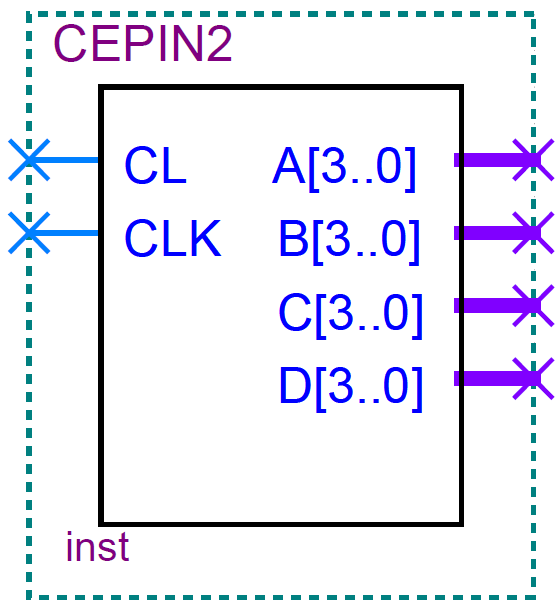
\includegraphics[width=0.3\textwidth]{picture/cepinfz.png} 
	\caption{}
	\label{fig:fengzhuangcepin}   
\end{figure}
\subsection{译码显示电路}
这一部分在EDA(II)中我是采用代码来完成的,但与同学交流后发现,使用原理图来搭建反而思路更清晰,因此在这里我尝试重新用原理图来完成译码显示部分。
\subsubsection{芯片搭建的译码显示电路原理}
显示译码电路用于数码管的动态显示,该实验需要8个显示管参与显示(2位频率控制字、2位相位控制字、4位测频显示),因此采用计数器74161设计模8循环计数;其输出作为4片74151的控制端,又作为3-8译码器74138的控制端。\par模8计数器的输出端a[0]、a[1]、a[2]连接到四片74151地址端,通过74151同时选取对应位进行输出,组成计时器某一位的BCD编码并接入显示译码器7447。\par与此同时,根据接入端的a[0]、a[1]、a[2],74138译码器也从8个数码管的使能端选择对应位有效,从而在对应数码管上显现一个有效数据。\par扫描的频率为1KHz,根据人眼的视觉暂留现象,会使人感觉到8个数码管在同时显示。
\subsubsection{译码显示模块}
译码显示电路的原理电路见图\ref{fig:yima},封装图见图\ref{fig:fengzhuangyima}。
\begin{figure}[hp]
	\centering  
	\includegraphics[width=\textwidth]{picture/yima.png} 
	\caption{}
	\label{fig:yima}   
\end{figure}
\begin{figure}[hp]
	\centering  
	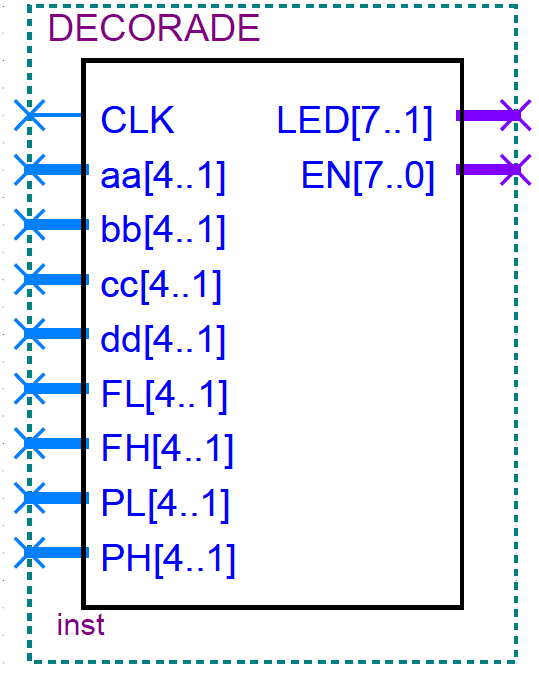
\includegraphics[width=0.3\textwidth]{picture/yimafz.png} 
	\caption{}
	\label{fig:fengzhuangyima}   
\end{figure}
\subsection{节省ROM}
在波形存储器中,所用的ROM有12位的地址线和10位的数据线,ROM中共有4096个数值。\par
但是正弦函数具有对称性,可以用$\frac{1}{4}$个周期的波形就能完整地表现出完整周期的波形:第二个$\frac{1}{4}$周期与第一个$\frac{1}{4}$周期波形是相位相反的关系,第三个$\frac{1}{4}$周期与第一个$\frac{1}{4}$周期波形是函数值相反的关系,第四个$\frac{1}{4}$周期与第一个$\frac{1}{4}$周期波形则是相位、函数值同时反相的关系。其关系如图\ref{fig:untitled}所示。
\begin{figure}[hp]
	\centering  
	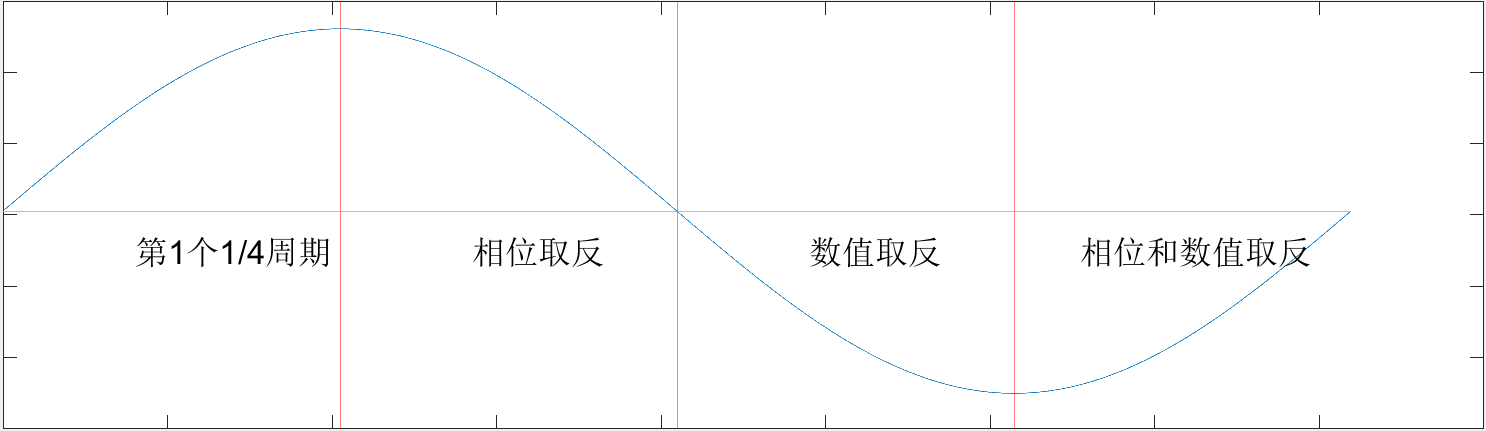
\includegraphics[width=\linewidth]{picture/untitled.png} 
	\caption{}
	\label{fig:untitled}   
\end{figure}
\subsubsection{取反电路}
借助ipm\_inv元件实现取反,电路原理见图\ref{fig:qufan},封装图见图\ref{fig:fengzhuangqufan}。
\begin{figure}[hp]
	\centering  
	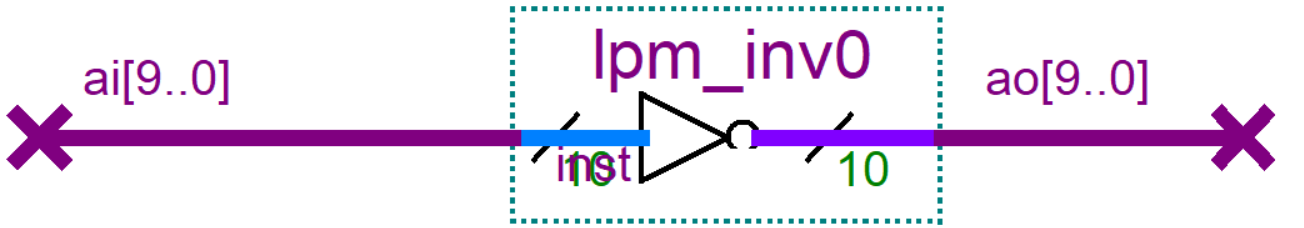
\includegraphics[width=0.7\textwidth]{picture/qufan.png} 
	\caption{}
	\label{fig:qufan}   
\end{figure}
\begin{figure}[hp]
	\centering  
	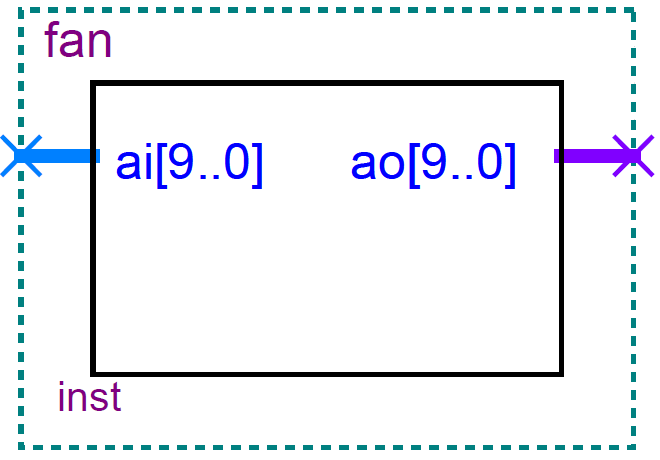
\includegraphics[width=0.3\textwidth]{picture/qufanfz.png} 
	\caption{}
	\label{fig:fengzhuangqufan}   
\end{figure}
\subsubsection{节省rom模块}
运用取反电路实现地址取反与输出取反,rom模块的电路原理见图\ref{fig:jies},封装图见图\ref{fig:fengzhuangjies}。
\begin{figure}[hp]
	\centering  
	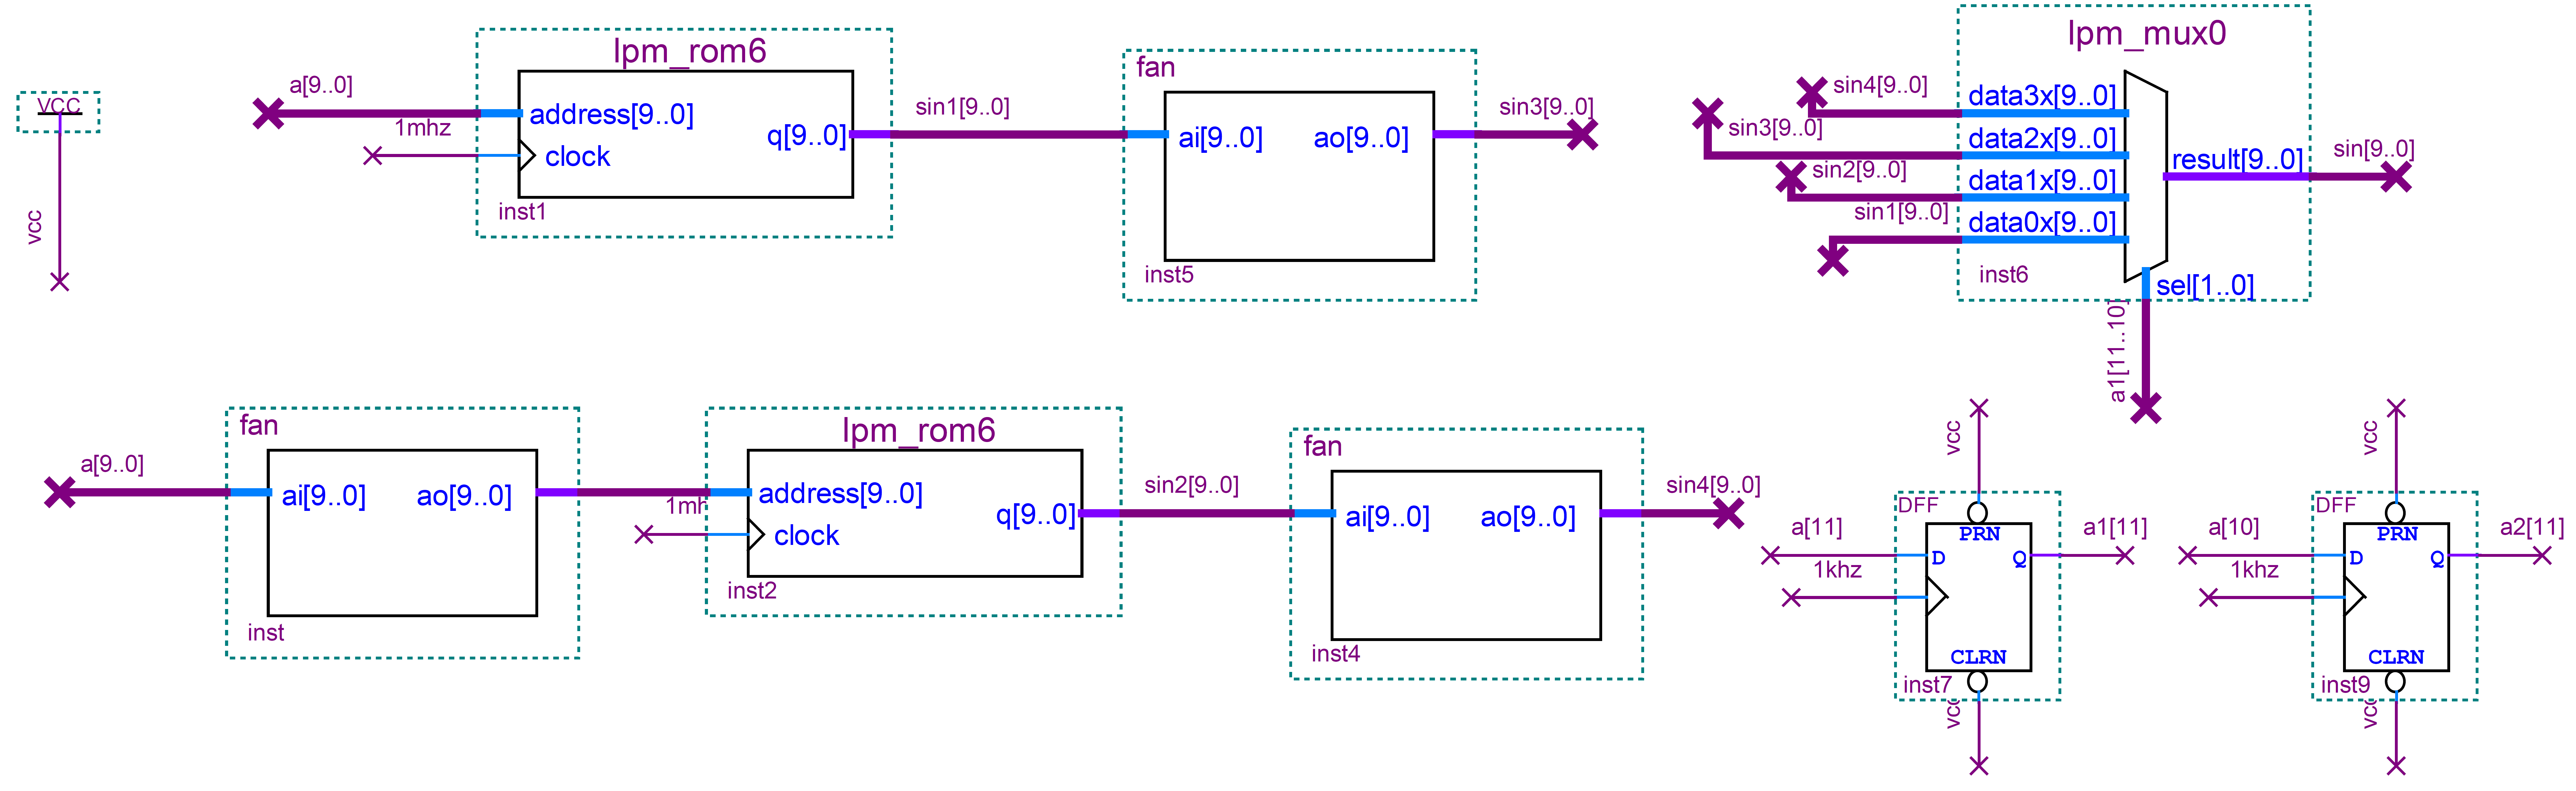
\includegraphics[width=\textwidth]{picture/jies.png} 
	\caption{}
	\label{fig:jies}   
\end{figure}
\begin{figure}[hp]
	\centering  
	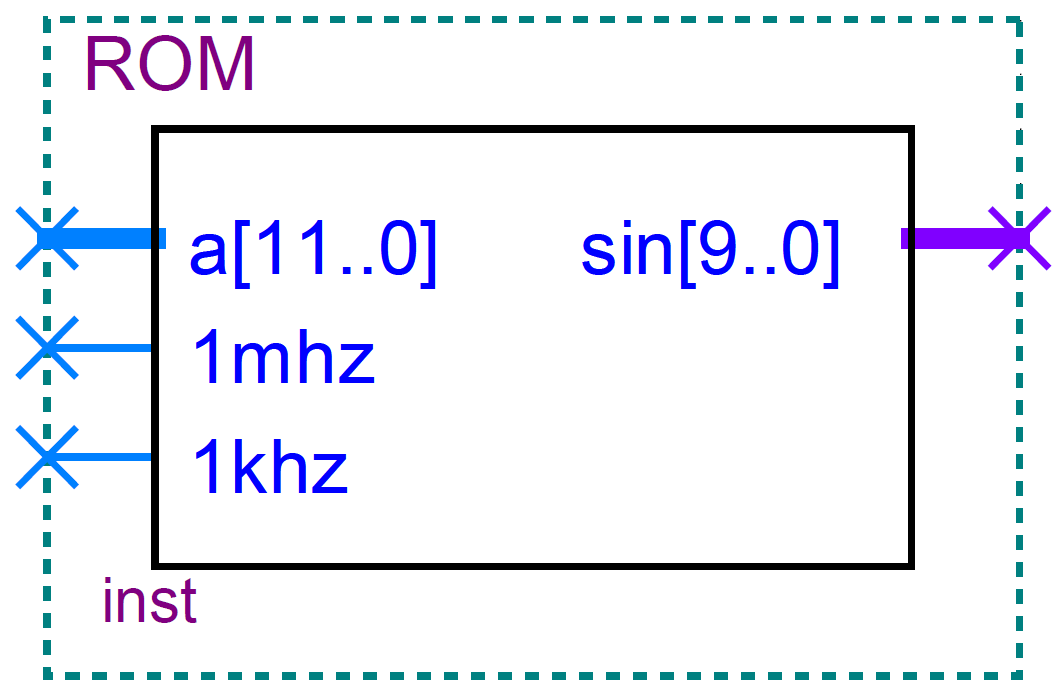
\includegraphics[width=0.3\textwidth]{picture/jiesfz.png} 
	\caption{}
	\label{fig:fengzhuangjies}   
\end{figure}
\subsection{AM调制}
信号调制是调制信号对载波的幅度、频率和相位进行变换。AM即标准调制信号,除了来自消息的基带信号外,还包含了直流信号,它是调制后输出信号既含载波分量又含边带分量的标准调幅信号。
\subsubsection{AM调制原理}
如图\ref{fig:119},在标准幅度调制器(AM)中,设载波信号为:$v_c(t)=V_{cm}cos{\omega_c}t$,调制信号为:$v_f(t)=V_{\Omega m}cos{\Omega}t$ .则标准调幅波信号为:
 $$v_{AM}(t)=[V_{cm}+v_f(t)]cos\omega_ct=(V_{cm}+V_{\Omega m}cos\Omega t)cos\omega_ct=V_{cm}(1+m_Acos\Omega t)cos\omega_ct$$
其中,$m_A=\frac{V_{\Omega m}}{V_{cm}}$被称为调幅度,是调幅信号的一个重要的参数,一般小于1,当$m_A$大于1时会出现过调幅。
\begin{figure}[hp]
	\centering  
	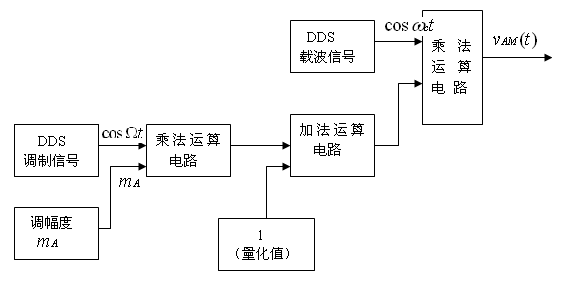
\includegraphics[width=0.8\textwidth]{picture/image119.png} 
	\caption{}
	\label{fig:119}   
\end{figure}
\subsubsection{AM模块}
AM调制电路原理见图\ref{fig:am},封装图见图\ref{fig:fengzhuangamfz}。
\begin{figure}[hp]
	\centering  
	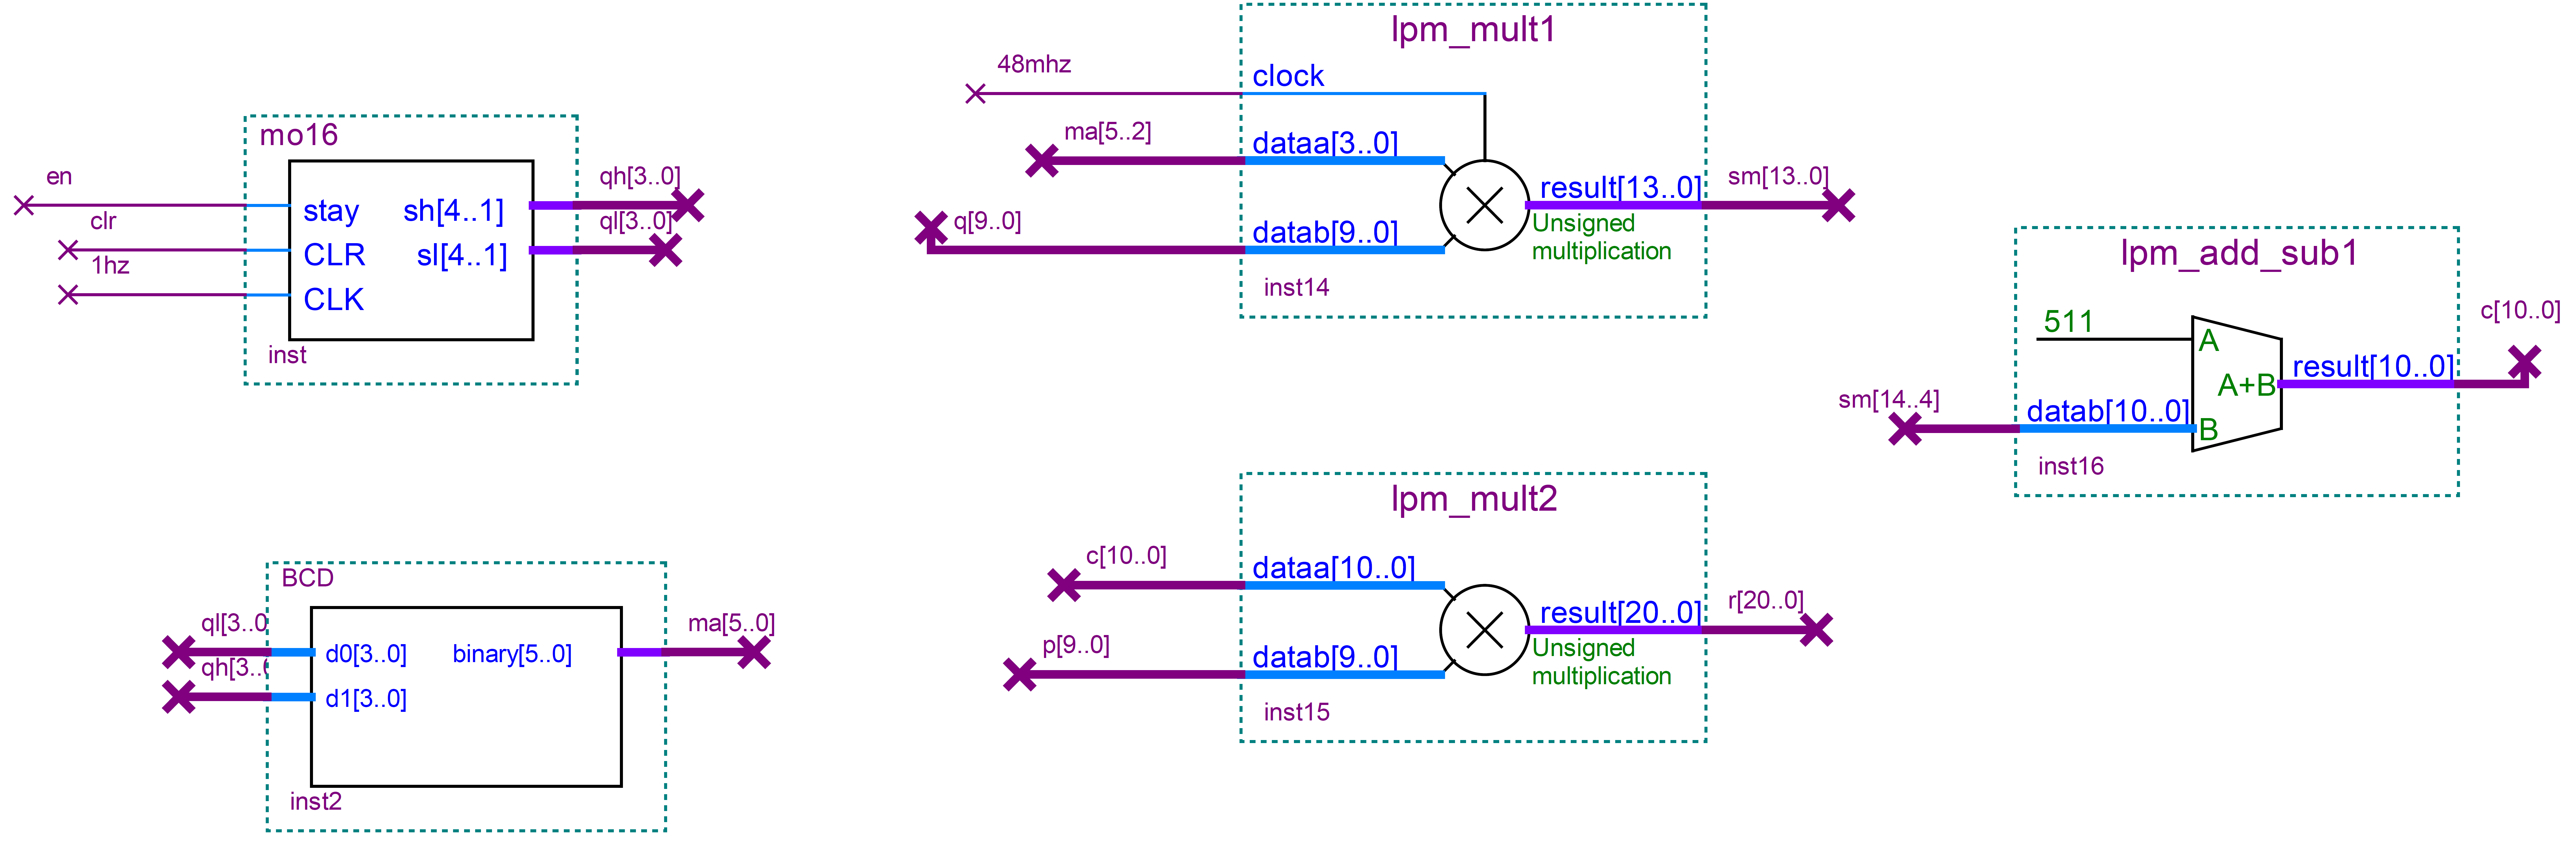
\includegraphics[width=\textwidth]{picture/am.png} 
	\caption{}
	\label{fig:am}   
\end{figure}
\begin{figure}[hp]
	\centering  
	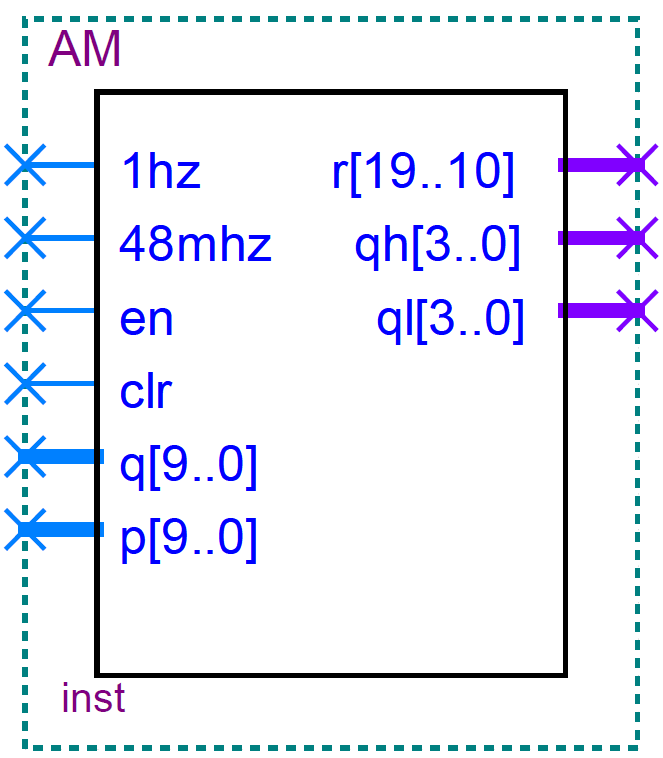
\includegraphics[width=0.3\textwidth]{picture/amfz.png} 
	\caption{}
	\label{fig:fengzhuangamfz}   
\end{figure}
\section{直接数字频率合成器总电路}
将以上几个模块相连,借助$IPM\_MUX$实现显示复用,通过逻辑门的组合实现开关复用,直接数字频率合成器总电路如图\ref{fig:all-2}。
\begin{lstlisting}[language=VHDL]

\end{lstlisting}
\begin{figure}[hp]
	\centering  
	\includegraphics[width=\textwidth]{picture/all.png} 
	\caption{}
	\label{fig:all-2}   
\end{figure}

\begin{lstlisting}[language=VHDL]
\end{lstlisting}
\section{调试、仿真、编程下载}
每个模块设计好之后都需要进行调试。调试可以帮助我们避免一些常见的小错误,如漏掉加电源VCC或接地GND等,或标注时不小心标注错误引脚不存在等。这样可以避免出现电路全搭完了但是结果出不来,不知道问题具体在哪的情况出现。这是最基本的检查,只能检查出一些语法运用的错误。\par然后还要对其进行波形仿真验证,来检查电路设计的正确与否,直至调试的仿真图完全正确为止,仿真得到的波形图在各个模块的论证时已经给出。 \par
波形仿真完成后,就要下载到实验箱上进行验收。下载方法比较繁琐,通常要设置一些程序的初始值、使能端等,但这是必须的一步,否则可能烧坏实验箱
上的某些原件,造成较大的损失。\par
将编译好的程序管脚分配,然后下载到实验系统中进行调试和验证。其中管脚分配如图\ref{fig:pins}。
\begin{figure}[hp]
	\centering  
	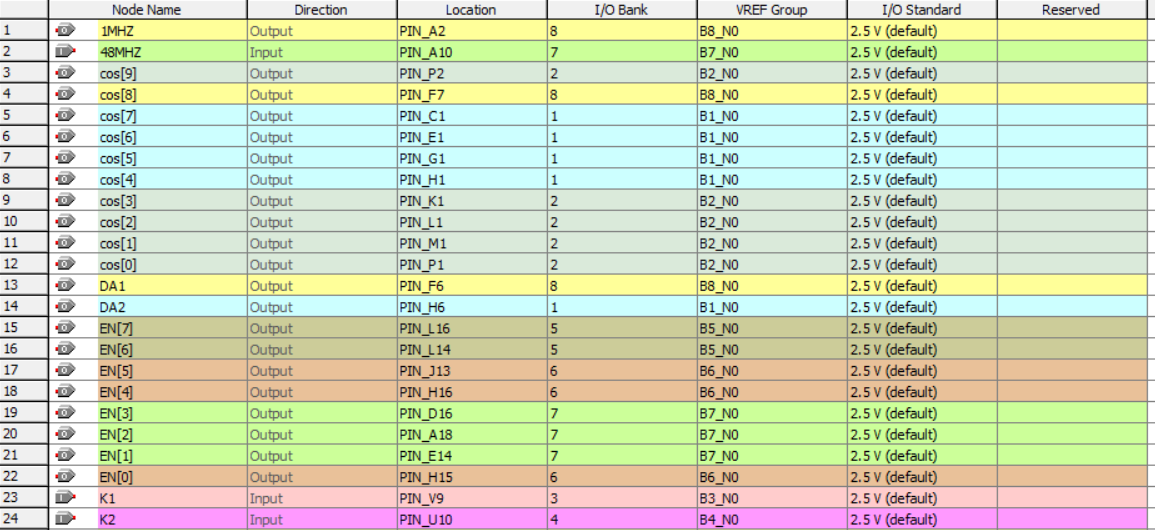
\includegraphics[width=\textwidth]{picture/pin1.png} 
	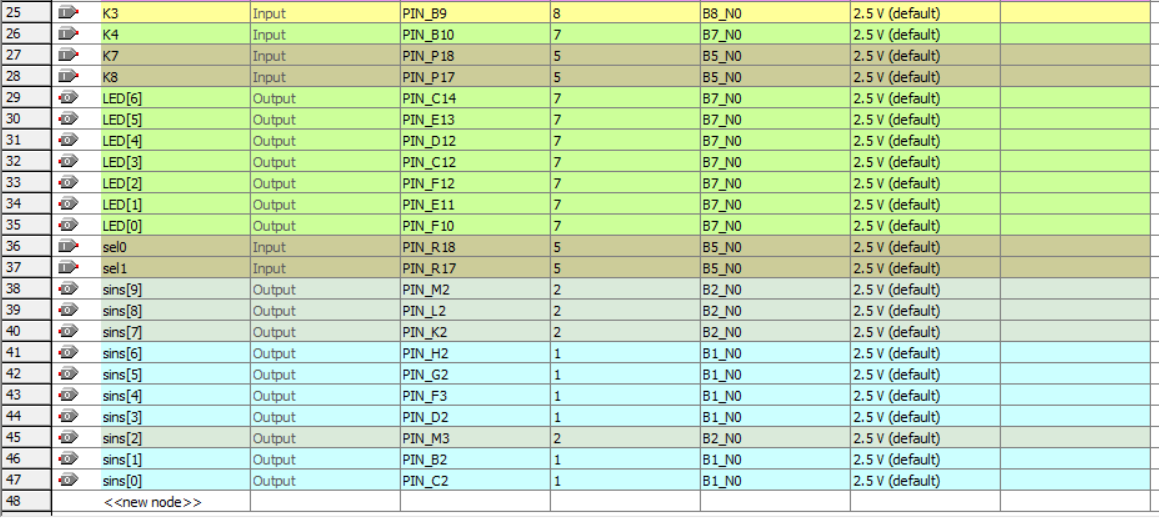
\includegraphics[width=\textwidth]{picture/pin2.png} 
	\caption{}
	\label{fig:pins}   
\end{figure}
\section{ 结论}
运行后可实现的功能有:
\begin{enumerate}[1、]
\item 开关全部置0时,频率控制字、相位控制字以1-39计数的方式输入,每秒自增,同时显示在数码管的左4位,前两位是频率控制字,后两位是相位控制字。示波器双路输出,共用频率控制字,相位控制字只对第一路起作用。第一路为用节省ROM实现的正弦波;第二路可由用户设定,开关全部置零时为方波。测频模块自动测量频率,并显示在数码管的右四位。
\item $K_1,K_2,K_3$组合起来进行频率控制字、相位控制字的使能与清零。具体实现如下:
\begin{enumerate}[(1)]
\item $K_1$是频率控制字/相位控制字选择开关:$K_1=0$时,$K_2,K_3$负责频率控制字;$K_1=1$时,$K_2,K_3$负责相位控制字;
\item $K_2$是使能开关:$K_2=1$时,频率控制字/相位控制字计数暂停;$K_2=0$时,频率控制字/相位控制字计数继续;
\item $K_3$是清零开关:$K_3=1$时,频率控制字/相位控制字计数清零;$K_3=0$时,频率控制字/相位控制字计数正常计数。
\end{enumerate}
\item $K_5,K_6$是波形选择开关:当$K_5,K_6$对应的二进制码为00时,输出方波;为01时,输出锯齿波;为10时,输出三角波;为11时,输出余弦波;
\item $K_4$是AM 调制开关:当$K_4=0$时,示波器第一路显示正弦波;当$K_4=1$时,示波器第一路显示调幅AM波,同时$K_7,K_8$开始起作用;
\item $K_7$是AM调制模块的调幅度控制开关:当AM调制开启,$K_7=0$时,AM调幅波的调幅度以16为周期,逐渐增大,又回到最小(通过模16计数器实现);$K_7=1$时,AM调幅波的调幅度保持不变;
\item $K_8$是AM调制模块的调幅度清零开关:当AM调制开启,$K_8=0$时,AM调幅波的调幅度正常计数;$K_8=1$时,AM调幅波的调幅度清零;
\item  测频电路能准确、稳定工作,当调整频率控制字稳定后,数码管能显示当前波形的频率,与示波器上所测得的频率基本一致,只有很小的误差。
\item 用节省ROM模块替换原ROM模块后,示波器上能检测到准确的正弦函数波形,相比较之前的ROM,改进后的ROM精度更高。
\end{enumerate}
\section{实验感想}
\subsection{实验过程中遇到的问题及解决问题的方法}
实验过程中遇到的问题主要有:
\begin{enumerate}[1、]
\item 在仿真总分频器时,由于采用了代码来实现,无法像上次一样去掉某一个分频来产生变化的波形了。我一度想用代码编各个分频器然后组合。经过同学的提醒明白了,因为各个频率的分频代码是一样的,只要保证分出1Mhz的分频没问题(这也是不要用长截止时间就可以仿真出来的),就可以认为分频没有问题。最终采用了这种方式验证。
\item 在设计测频电路的时候,原本我是想用VHDL语言进行设计的,但设计的过程并不顺利,并且因此浪费了很多时间,最后只能选择用电路图的方法搭建测频电路。
\item 在下载到实验箱运行时也出现了问题,再次出现了实验板上没有任何显示的情况。有了上次的经验,我一开始就检查管脚的分配,发现又是管脚分配有问题,改正这个错误后,就显示出来了。
\item 做节省ROM时有毛刺出现,毛刺出现的原因是在输出$\frac{\pi}{2}-\pi$的波形时,是从$0-\frac{\pi}{2}$的第一个点开始取反的,这个时候波形输出从最高点一下落到最低点导致出现了毛刺。通过查阅相关的书籍以及文献资料,我决定采用两个D触发器实现延时,从而避免了毛刺的出现。
\item 在做提高功能AM调制时,也遇到了不少的问题。在一开始的时候,没有考虑到载波信号频率应该要比调制信号的频率大得多,所以调制出来的波形一直都不理想,后来经过向同学请教,找到了这个问题,并作了相应的修改,从而解决了这个问题。
\end{enumerate}
\subsection{实验的收获与感受}
这是第二次使用QuartusII做电路设计,老师一开始只讲了一些基本原理以及需要注意的事项,并没有给具体的思路,需要我们另外查阅相关的资料进行设计。由于在前一周完成了多功能数字钟的设计实验,这一周再参加这个直接数字频率合成器设计的实验明显感觉有所不同,设计过程中自己也不再像上一周那样那么的迷茫。同时,我对VHDL语言的使用也更得心应手,大大降低了设计的工作量。\par完成这个实验,必须要对电路的总体框架有一个大概的把握,需要用到什么功能、设计什么模块,都是需要提前考虑的。\par
电路系统圆满完成了要求的基本功能,基础模块主要包括分频、控制字/相位字产生、进制转换、累加器、测频、显示译码等内容。\par与第一个实验相比较,没有涉及到的就是累加器,需要额外设计,除了测频电路,其他模块相对来说是比较容易实现的。
而显示译码模块部分,我在EDA(II)中用的是代码,但是与同学交流后发现,电路图搭建反而更直观,因此本实验用了电路图来实现。\par
在此基础上,我实现了更大范围的频率控制字与相位控制字、双路输出、节省ROM电路模块以及输出三角波、方波、锯齿波等多种波形、AM调制等拓展功能的设计。而在设计节省ROM电路模块的时候,发现正弦输出有毛刺的问题,在查阅资料后得到了解决的方案。\par
这次设计实验中,
我意识到只要有了正确的设计思路,设计电路时考虑全面,遇到问题一步一步地解决,是可以实现想实现的功能的。\par
而在原理图搭建好之后下载到试验箱的过程中,一定要仔细分配管脚,要看清楚,不能填错,要和电路对应好。检查时要耐心,有条不紊地进行,不能急于求成。\par
最后,非常感谢老师和周围同学在本次实验中给我的帮助,让我受益匪浅。这次实验, 我再次体验到了设计数字逻辑电路的不易与乐趣,大大激发了我动手实践的热情。希望有机会能多多尝试做做电路设计。相信这次实验也会给今后的学习和生活带来帮助。
\subsection{期望及要求}
这次实验的结果总体也还算圆满,但同样存在一些小小的遗憾。实验中设计测频电路的时候,我原本计划用VHDL语言进行设计,但设计的过程并不顺利,最后只能选择电路图的方法,希望有机会能研究出来。
\par这次实验,使我对于调制的理解更加深刻,有机会希望能完成其他形式的调制电路的设计。
\begin{thebibliography}{15}\zihao{4}\addtolength{\itemsep}{-0.5ex}\addcontentsline{toc}{section}{参考文献}
\bibitem{1}数字逻辑电路与系统设计.蒋立平.北京:电子工业出版社,2008.7 
\bibitem{} VHDL数字电路设计教程.佩德罗尼.北京:电子工业出版社, 2013.1
\bibitem{} 晏细兰,谢景明,熊茂华.基于FPGA和VHDL的高精度数字频率计研究与设计[J].计算机光盘软件与应用,2014,17(15):91-94.
\bibitem{} 谢煜 ,黄为.一种基于VHDL语言数字频率计的设计与实现[J].电子设计应用,2003(07):25-27.
\end{thebibliography}
\end{document}
